\documentclass[a4paper,11pt]{article}
%在此可进行页面设置
%\textwidth=14cm
%\textheight=22cm
\usepackage{tikz}
\usetikzlibrary{mindmap,trees}
\usepackage{verbatim}
\usepackage{float}
\usepackage{pdfpages}
\usepackage[section]{placeins}
\usepackage{setspace}%使用间距宏包
\usepackage[76620]{MCMPackage}  %队号在这里填写
%\usepackage[XXX,nosheet]{MCMPackage}%这个参数形式可去掉summary sheet首页。
\problem{C}  %选题

\title{Energy Compact Focused On Interstate Energy Structure}%在此插入论文标题
\date{February 12, 2018}

%设置段落之间的距离,若不需要删除或者注释掉即可。
\setlength\parskip{.5\baselineskip}

%为了首行缩进
%\usepackage{indentfirst}
%\setlength{\parindent}{2em}

\makeatletter
\def\@cite#1#2{\textsuperscript{[{#1\if@tempswa , #2\fi}]}}
\makeatother

%设置参考文献的小上标
\begin{document}
%摘要
\begin{abstract}


\par With the depletion of existing energy on the planet, the usage of energy especially renewable energy (REU) has become a more and more widespread concern. This paper establishes a series of models to help govenors understand the REU among four states and build interstate energy compact.

\par In the \textbf{\emph{Energy Profile Model}}, we analyze each state's own energy profile based on factors such as the proportion of renewable energy and the weight of the primary energy, along with the main sectors in which energy be consumed. Through analyzing the classification criteria of MSN, we \textbf{\emph{dig into the data}} and get production and consumption of each kind of energy, which represent the energy's usage in sectors or in total, and the correlation coefficient between them is taken as a factor of factor analysis method, then we calculate and simulate the whole model and get the results.

\par Based on the Energy Profile Model, we take time dimension and the specific relationship between sectors and energy category into consideration to obtain the evolution of energy profile in each state from 1960 to 2009, which is called the \textbf{\emph{Profile Evolution Model}}. \textbf{\emph{Energy Usage Comparison Model}} is established to get the score of state REU, and renewable energy usage of different sectors in different states (REUSS) is considered in the AHP (The analytic hierarchy process) as the influencing factor. The higher the score of the AHP result is, the better the state of renewable energy is in use. The REUSS change in the time dimension is integrated to analyze the similarities and differences in REU among states.

\par The purpose of the \textbf{\emph{Best Profile Analysis Model}} is to determine the best performing profile among the REU profiles in each state. In this model, we have considered various factors including the total amount of REU, per capita REU and the gradient of two kinds of REU. Based on the calculation and comparison of previous model, we choose a best profile from the comprehensive factors.

\par \textbf{\emph{Prediction Model}} predicts the energy profile of each state in 2025 and 2050 based on the Profile Model and Evolution Model. Based on the results obtained from the previous models, a regression curve is fitted using the nonlinear regression equation to predict future trends. Our forecast is based on the regression of time periods between the mutation point caused by factors such as the policy change before 2009 to the present and assumes that there are no factors such as policy that can cause sudden changes in the coming period.

\par Based on the analysis of all the above models, we establish a \textbf{\emph{REU Targets Determining Model}} which predicts the change of total energy usage using a linear regression model and predicts the energy profile using the Prediction Model, and then specifies the target of REU for 2025 and 2050. By determining REU targets, we can help governors set the goal of interstate energy compact.

\textbf{Keywords:  Renewable Energy; Comprehensive Factors; Analytic Hierarchy Process; Data Characteristics Analysis}

\end{abstract}
\maketitle%插入标题
\thispagestyle{empty}%本页不遍页码

\newpage%另起一页插入目录
\thispagestyle{empty}%防止目录两页而出现一页带页码
\begin{spacing}{0.5}%%行间距变为single-space
\tableofcontents%目录
\maketitle
\thispagestyle{empty}
\end{spacing}

\newpage%另起一页书写正文
\pagenumbering{arabic}%开始编页码(阿拉伯数字)

\section{Introduction}
%In reference \cite{RefB}.%引用参考文献

\subsection{Background}
    
\par Nowadays, with the development of technology and the deterioration of the environment, many countries, especially the United States, began to value the renewable energy, such as wind energy and geothermal energy. Meanwhile, traditional energy, such as gasoline and coal, still plays an important role in economics. And it is obvious that the usage of the renewable energy will support the future of mankind.
\par In the United States, an interstate compact is an agreement between two or more states. Frequently, these agreements create a new governmental agency which is responsible for administering or improving some shared resource such as a seaport or public transportation infrastructure.\cite{1} In 1970, the Western Interstate Energy Compact was formed, which was devoted to foster cooperation to develop and manage the nuclear technology. Recently, California, Arizona, New Mexico, and Texas wish to form a new interstate energy compact focused on increased usage of renewable energy sources. 
\par A data file provides 50 years of data in 605 variables on each of these four states' energy production and consumption, along with some demographic and economic information. In order to inform a set of goals for the new interstate energy compact, we will analyze the given data and model.


\subsection{Problem Restatement}
%这一部分写问题分析以及我们要解决的问题
\subsubsection{Part \uppercase\expandafter{\romannumeral1}}
\par For Problem A, in order to lay the foundation of analyzing, we are required to create an energy profile for each of the four states. Meanwhile, the profiles should be created on the analysis of the given data.

\par For Problem B, it adds a factor of consideration to the time dimension based on question A. Especially, the type of energy that needs to be analyzed becomes renewable energy, and the focus shifted from within a single state to between states. Explaining briefly the similarities and differences.

\par For problem C. To determine the best performing profile among the REU profiles in each state in 2009, we need to inspect the comprehensive factors based on the calculation and comparison of previous model.

\par For Problem D, in order to predict energy profile of usage of each state in 2025 and 2050, we need to base on the results of Problem A, B, C and the given data to establish regression equations or other models.

\subsubsection{Part \uppercase\expandafter{\romannumeral2}}

\par It is suggested in the Problem A that we should determine targets based on the problems of Part \uppercase\expandafter{\romannumeral1} of the renewable energy usage for the four states in the year of 2025 and 2050. 

\par For Problem B, we are supposed to give some suggestions to the governors, so that they will know the actions they should take to meet the goals.

\subsubsection{Part \uppercase\expandafter{\romannumeral3}}
\par On the basis of the analysis and models in the two parts before, we prepare the state profiles of 2009, our predictions towards energy usage and some recommendations on adopting goals for the energy compact.


\section{Assumptions}
\begin{enumerate}%[(1)]
\renewcommand{\labelenumi}{(\theenumi)}
    \item In factor analysis, we suppose the corresponding valuables as the main factors when the cumulative percentage is over 0.65.
    \item When we do regression analysis, we suppose that F-test or t-test is passed if the Pr of them is less than 0.05.
    \item When we do regression analysis, we suppose that effect of regression is good if $R^{2}$ is greater than 0.65.
\end{enumerate}


\section{Symbol Description}
%符号说明
In the section, we use some symbols for constructing the model as follows.

\begin{center}
\begin{tabular}{cc}%r 表示表格内文本右对齐;c表示居中对齐;l表示左对齐;| 表示竖铅直线
    \toprule[2pt]
    \textbf{Symbol} & \makecell[c]{\textbf{Description}}\\
    \hline
$R$&The correlation coefficient matrix of natural gas, electricity, petroleum products and coal.\\ 
$\lambda_i$&The eigenvalue of R, i=1,2,3,4.\\
$U$&The Eigenvector matrix for the eigenvalues of R.\\ 
$A$&The factor loading matrix.\\
$f_i$&Factor, i=1,2.\\ 
$w_1$&The weight of natural gas.\\ 
$w_2$&The weight of electricity.\\ 
$w_3$&The weight of petroleum products.\\ 
$w_4$&The weight of coal.\\ 
$\eta_1$&The proportion of renewable energy in total energy.\\
$\eta_2$&The proportion of different sector in renewable energy usage.\\
$Y$&The level of renewable energy usage.\\ 
$X_i$&Transportation(i=1), commerce(i=2), electricity(i=3), industry(i=4), resident(i=5), i=1,2,3,4,5.\\ 
$C,B_i$&The pairwise comparison matrixs, i=1,2,3,4,5.\\
$\beta,\beta_i$&weight vectors, i=1,2,3,4,5.\\
$Z_i$&The score based on the total renewable energy usage of the four states, i=1,2,3,4.\\
$S$&The amount of the total renewable energy usage of the four states.\\ 
$S_i$&The amount of the total renewable energy usage of each of the four states, i=1,2,3,4.\\

% $T_n$&The discrete time series of the node checking information.\\ 
% $p_{in}$& The probability of ~$Node~i$~ to check information at the moment of $T_n$.\\
% $q_{in}$&The probability that information is able to continue to spread\\
% $\lambda_i$&The probability of node's retransmission or comments after receiving the message.\\
% $N_n$& The number of nodes that have received information at the moment ~$T_n$~\\
% $Q_n$& The number of nodes that have received information at the moment ~$T_n$~\\
% $\gamma_i$& The new attention degree of a certain node in the unit time ~$\Delta t$~\\
% $D_i$&The degree of ~$Node~i$~\\
% $C_i$&The clustering of ~retransmission~$Node~i$\\
% $L_{ij}$&The shortes path length of ~$Node~i$~ and ~$Node~j$\\
    \bottomrule[2pt]
    %以下两条指令此处不用
    %\caption{表格标题}
    %\label{标签名}%便于交叉引用
\end{tabular}
\end{center}



\emph{P.S: Other symbol instructions will be given in the paper.}


% 4
\section{Energy Analysis Model}

% \par We divide 
% \par Factor Analysis is a multivariate statistical analysis method, which is based on the internal dependencies of the correlation matrix of the indicator. It attributes some of the variables that have complex relationship to a few irrelevant factors.\cite{2} We will use this method to deal with problem A in the section.

% 4.1
\subsection{Distinction approach of energy construction}
% 4.1.1
\subsubsection {MSN character analysis}

\par By observing the given data and acquiring knowledge from Appendix A. Mnemonic Series Names (MSN)\cite{3}, we can conclude that the MSNs are usually five-character codes, and the three parts of the characters generally represent the following meanings.

\begin{itemize}
    \item First and second characters: describes an energy source (for example, NG for natural gas, MG for motor gasoline);
    \item Third and fourth characters: describes an energy sector or an energy activity (for example, RC for residential consumption, PR for production);
    \item Fifth character: describes a type of data (for example, P for data in physical unit, B for data in billion Btu).    \cite{3}
\end{itemize}

\par As described above, the first part and the second part of the MSN code represent for certain specific meanings. However, in our analysis process, we are more concerned about the general classification of these MSN codes. 

\begin{figure}[h]%[!hptb]
    \centering 
    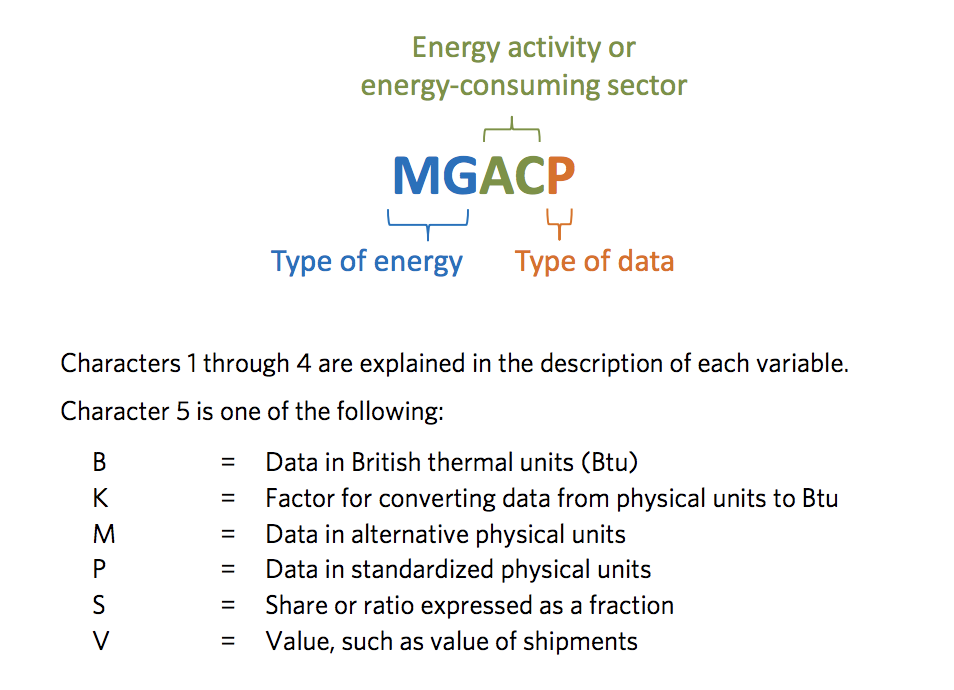
\includegraphics[width=0.65\textwidth]{./Pic/msn_5.png}
    % 图片标题
    \caption{The meaning of a MSN code, emphasizing the fifth character. Reference \url{https://www.eia.gov/state/seds/sep_use/notes/use_a.pdf}}
    \label{fig:msn_5}  
\end{figure}
\par We also found that the fifth character has six values at most, which can be seen in figure \ref{fig:msn_5}. Thus we start to focus more on the analysis of the fifth character. After comparing the units of the six and calculating, we find the relationship between these six symbols are
\begin{equation}
    B=KP~~~~~,~~~~~V=BD / 1000
\end{equation}

\par From the equation we can get the conclusion that B is a key factor between the two equations and can build a connection between them. And we find that all MSNs whose fifth character is B have the same unit Billion Btu, which can be an excellent representative of the MSNs who have the same prefix. So we filter the 605 MSNs and find 215 MSNs' suffix is B. At this stage we have reduced the 605 kinds of MSNs into 215. Every kind of the 215 MSNs contains several MSNs with different suffix but the same prefix.


% 4.1.2
\subsubsection {MSN classification analysis by energy unit}


\par In order to classify the 215 MSNs more clearly, we look into everyone of the division and find that a large percent of the kinds have the suffix P, which represents the standardized physical units. Physical units naturally represent for the energy classification in the real physical world, and there are mainly \textbf{4 kinds of standardized physical units} in the data set as can be seen in figure \ref{tab:energy-unit}, so it is reasonable to classify the data into 4 groups according to the units.
% \par According to the analysis above, we suppose the four units as the following representatives.

\begin{table}[H]
    \centering
    \begin{tabular}{|c|c|}
        \hline Energy name & Unit\\
        \hline Petroleum products & Thousand barrels\\
        \hline Coal & Thousand short tons\\
        \hline Electricity & Million kilowatthours\\
        \hline Natural gas & Million cubic feet\\
        \hline
    \end{tabular}
    \caption{Energy name and unit reference table}
    \label{tab:energy-unit}
\end{table}


% \par Fule oil related MSN are: ABICP, ARICP, ARTCP, ARTXP, AVACP, AVTCP, AVTXP, CLTXP, COICP, DFACP, DFCCP, DFICP, DFRCP, DFTCP, DFTXP, DKEIP, EMTCP, ENACP, ENCCP, ENICP, ENPRP, ENTCP, ESTXP, FNICP, FOICP, FSICP, JFACP, JFTCP, JFTXP, JKACP, JKTCP, JNACP, JNTCP, KSCCP, KSICP, KSRCP, KSTCP, KSTXP, LGACP, LGCCP, LGICP, LGRCP, LGTCP, LGTXP, LUACP, LUICP, LUTCP, LUTXP, MBICP, MGACP, MGCCP, MGICP, MGTCP, MGTXP, MSICP, NAICP, P1ICP, P1TCP, P1TXP, PAACP, PACCP, PAEIP, PAICP, PAPRP, PARCP, PATCP, PATXP, PCCCP, PCEIP, PCICP, PCTCP, PLICP, POICP, POTCP, POTXP, PPICP, RFACP, RFCCP, RFEIP, RFICP, RFTCP, RFTXP, SGICP, SNICP, UOICP, USICP and WXICP;
% \par coal related MSN are: CCEXP, CCIMP, CCNIP, CLACP, CLCCP, CLEIP, CLICP, CLKCP, CLOCP, CLPRP, CLRCP and CLTCP;
% \par Electricity related MSN are: ELEXP, ELIMP, ELNIP, ESACP, ESCCP, ESICP, ESRCP, ESTCP, GEEGP, HYCCP, HYEGP, HYICP, HYTCP, HYTXP, NUEGP, NUETP, SOEGP and WYEGP;
% \par Natural gas related MSN are: NGACP, NGCCP, NGEIP, NGICP, NGLPP, NGMPP, NGPZP, NGRCP, NGTCP, NGTXP and NGVHP.


% \par \textbf{fule oil}: Thousand barrels;
% \textbf{coal}: Thousand short tons;
% \textbf{electricity}: Million kilowatt-hours;
% \textbf{natural gas}: Million cubic feet.

% \begin{figure}[!h]%[!hptb] 
%     \centering 
%     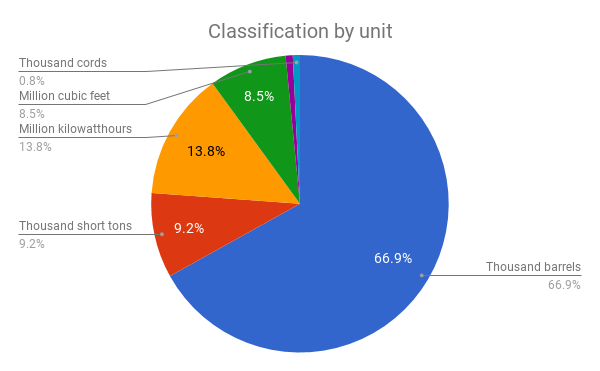
\includegraphics[width=0.8\textwidth]{./Pic/classification_by_unit.png}
%     \caption{Classification by unit in the suffix P.}
%     \label{fig:classification_by_unit}  
% \end{figure}

% 4.2
\subsection{Factor analysis function}

\par There are many relationships among MSNs. In order to simplify the complex dependencies between the four energy classification, we used factor analysis to establish an optimal model to analyze the actual weights of the four types of energy sources.

% \par According to the Formula in the Table A1.Consumption Variables,\cite{4} we remove variables that can be obtained by addition and subtraction of other variables so that we can avoid the repeat of variables when we calculate the correlation coefficient matrix. 
% \begin{enumerate}[Step 1:]
% \item Standardize data samples.

% \item Calculate the correlation matrix R of the sample.

% \item Find the eigenvalues and eigenvectors of the correlation matrix R.

% \item According to the cumulative contribution rate of the system to determine the number of the main factor.

% \item Calculate the factor load matrix A.

% \item Determine the factor model.

% \item Based on the above calculation results, the system is analyzed.
% \end{enumerate}

\par Through analyzing the given data and calculation, we can obtain R, the correlation coefficient matrix of natural gas, electricity, petroleum products and coal.
\begin{equation}
    \centering
R=\begin{pmatrix} 1 & r_{12} & r_{13} & r_{14} \\ r_{21} & 1 & r_{23} & r_{24} \\ r_{31} & r_{32} & 1 & r_{34} \\ r_{41} & r_{42} & r_{43} & 1\end{pmatrix}
\end{equation}


\par Then we can obtain the eigenvalues of R
\[
\lambda_1, \lambda_2, \lambda_3, \lambda_4
\]
and they must under the limit of
\[
    \lambda_1 \geqslant \lambda_2 \geqslant \lambda_3 \geqslant \lambda_4
\]
\par Meanwhile, we obtain the eigenvector matrix for the eigenvalues of R, U[ ,i] is the eigenvector of $\lambda_i$.
\begin{equation}
    \centering
U=\begin{pmatrix} U[ ,1] & U[ ,2] & U[ ,3] & U[ ,4]\end{pmatrix}
\end{equation}
\par Simply, the overall percentage and cumulative percentage of eigenvalues are as follows.
\begin{table}[!hbp]
    \centering 
    \begin{tabular}{|c|c|c|}
\hline
Eigenvalue & Overall percentage & Cumulative percentage \\
\hline
$\lambda_1$ & a1 & a2 \\
\hline
$\lambda_3$ & b1 & b2 \\
\hline
$\lambda_4$ & c1 & c2 \\
\hline
$\lambda_2$ & d1 & d2 \\
\hline
\end{tabular}
\caption{Percentage}
\end{table}
\par We choose the two main factors that are satisfied with assumption 1. Then we take out their corresponding eigenvectors from U, and we can obtain the factor loading matrix
\begin{equation}
    \centering
A=\begin{pmatrix} a_{11} & a_{12} \\ a_{21} & a_{22} \\ a_{31} & a_{32} \\ a_{41} & a_{42}\end{pmatrix}
\end{equation}
the first row of A is
\begin{equation}
    \centering
\sqrt{\lambda_1} \times U[ ,1]
\end{equation}
the second row of A is
\begin{equation}
    \centering
\sqrt{\lambda_3} \times U[ ,3]
\end{equation}

% 4.2.1

\par According to the factor loading matrix A, we can get the factor analysis model is
\begin{equation}
    \centering
    \text{natural gas}=a_{11} \times f_1+a_{12} \times f_2
\end{equation}
\begin{equation}
    \centering
    \text{electricity}=a_{21} \times f_1+a_{22} \times f_2
\end{equation}
\begin{equation}
    \centering
    \text{petroleum products}=a_{31} \times f_1+a_{32} \times f_2
\end{equation}
\begin{equation}
    \centering
    \text{coal}=a_{41} \times f_1+a_{42} \times f_2
\end{equation}
\par The definition of the weight of variables is\cite{5}
\begin{equation}
    \centering
w_i=\frac{ \theta_i }{ \sum_{i=1}^{4}\theta_i } \times 100\%
\end{equation}
\begin{equation}
    \centering
\theta_i=A[i,1] \times \lambda_1+A[i,2] \times \lambda_2+A[i,3] \times \lambda_3+A[i,4] \times \lambda_4
\end{equation}

\par Therefore, we can obtain the weights of natural gas, electricity, petroleum products and coal, which are between 0\% and 100\%.

\[
w_1, w_2, w_3, w_4.
\]

% 4.2.2
\subsubsection{Profiles of four kinds of energy}

\par From the point of the factor analysis model, we can easily find that $f_1$ is a positive factor for natural gas, petroleum products, coal, and a negative factor for electricity. Meanwhile, $f_2$ is a positive factor for coal, and a negative factor for natural gas, electricity, petroleum products. 
    So we can obtain the weights of variables of the four states in 2009 as the following figure:

\begin{figure}[H] 
    \centering 
    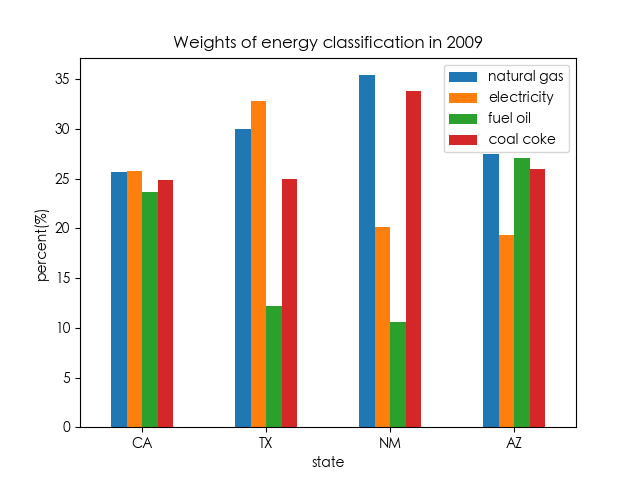
\includegraphics[width=0.7\textwidth]{./Pic/1-1.png}
    \caption{Weights of energy classification in 2009}
    \label{fig:1-1}
\end{figure}

\par According to figure \ref{fig:1-1}, the contribution rates of the four kinds of energy are very close in California. But in New Mexico and Texas, natural, electricity, and coal are main energy, because the addition of their contribution rates is over 85\%. And in Arizona, the contribution rate of electricity is less than the other energy. 

% 4.3
\subsection{Renewable energy profile}

\par In the previous section, we have set up a good factor analysis model for energy classification. It doses help us build the profile of the states' energy, but it dosesn't pay much attention to the difference between renewable energy and non-renewable energy. So in this part, we analyze the data set and give the profile of renewable energy in four states.

% 4.3.1
\subsubsection{Renewable energy usage percentage}
\par To get a preliminary understanding of the renewable energy usage in four states, we decide to get the proportion of renewable energy in total energy in the first step.

\par What's important is that we find that there are some specific MSNs and formulas in the reference \cite{4} which can describe the usage of renewable energy clearly and precisely. MSN \textbf{RETCB} is a good example, which represents renewable energy sources total consumed in a state.
\par Then we search for the MSN in the given data and find every state have this MSN. 
So this is indeed the representative MSN variable of the usage of renewable energy in every state. And then we find the \textbf{TETCB} MSN stands for the total energy consumed in a state. So we get the equation:

\begin{equation}
    \eta_1=\frac{\text{RETCB}}{\text{TETCB}}
\end{equation}

\par After calculating with the formula, we get the results of $\eta_1$, which can be seen in figure \ref{fig:1-2}

\begin{figure}[H]%[!hptb] 
    \centering 
    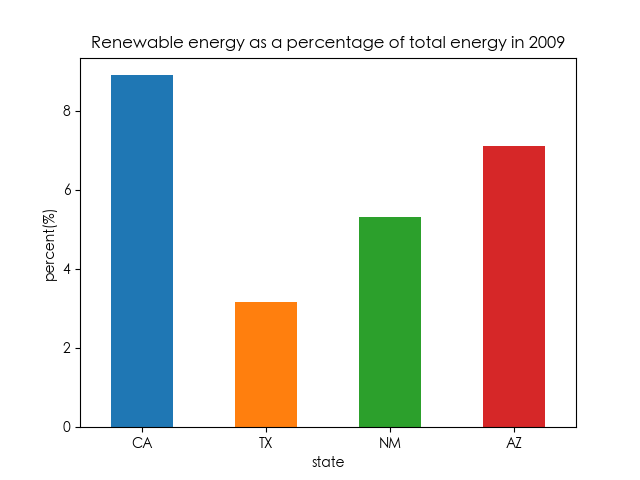
\includegraphics[width=0.7\textwidth]{./Pic/1-2.png}
    % 图片标题
    \caption{The proportion of renewable energy in total energy of four states in 2009.}
    \label{fig:1-2}  
\end{figure}
% 4.3.2
\subsubsection{Renewable energy usage in different sectors}
\par There are many factors that influence the usage of energy in a state. So it is reasonable to search for the situation of renewable energy usage in the different sector in every state.
\par Similar to the previous section, we find that there are some MSNs that describe the renewable energy in certain sector and formulas that calculate the value of it. 
Take transportation sector, for example, MSN \textbf{REACB} stands for renewable energy sources consumed by the transportation sector, so the sector's percentage in renewable energy consumption can be calculated through the formula. 

\begin{equation}
    \eta_2=\frac{\text{REACB}}{\text{RETCB}} \times 100\%
\end{equation}

\par After calculating with formulas, we get the results of $\eta_2 $, which can be seen in table \ref{tab:1-3}.

\begin{table}[!htb]
    \centering
    \begin{tabular}{|c|c|c|c|c|c|}
        \hline state & transportation & commercial & electric power & industrial & residential\\
        \hline CA & 1.433165353\% & 75.54688353\% & 4.482754103\% & 3.681370998\% & 11.33704864\%\\
        \hline TX & 1.199750149\% & 58.85661983\% & 15.73747739\% & 5.531569236\% & 18.44472327\%\\
        \hline NM & 4.3751358\% & 51.12013584\% & 6.997275293\% & 25.40469112\% & 11.30993476\%\\
        \hline AZ & 1.45721187\% & 62.71113276\% & 4.796738813\% & 8.130332086\% & 18.46557951\%\\
        \hline
    \end{tabular}
    \caption{The weights of variables of the four states in 2009}\label{tab:1-3}
\end{table}

% \begin{figure}[h]%[!hptb] 
%     \centering 
%     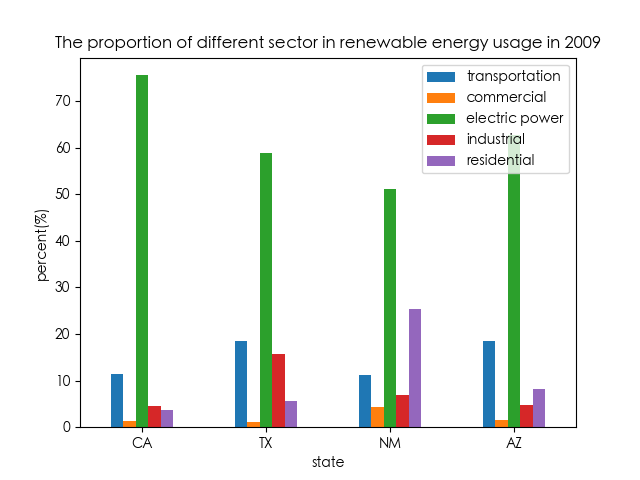
\includegraphics[width=0.6\textwidth]{./Pic/1-3.png}
%     % 图片标题
%     \caption{The proportion of different sector in renewable usage of four states in 2009.}
%     \label{fig:1-3}  
% \end{figure}


% 5
\section{Profile Evolution Model \& Energy Usage Comparison Model}


\par We have set up a good model for energy profile evaluation (State Energy Analysis Model) to analyze the energy profile of each state in a given year. 
\par The profile evolution model takes \textbf{time factor} into consideration to get the energy profile evolution results of four states. Besides,
we will use a new model Analytic Hierarchy Process (AHP) to deal with the analysis of possible influential factors of similarities and differences among the four states.

% 5.1
\subsection{Profile Evolution Model}
\par On the basis of the energy profile model, we try to bring time factor into the model and get the evolution result of the profile. 

% 5.1.1
\subsubsection{Model improvement with time factor}
\par Along with how to bring time factor into the model, we have a basic solution of calculating the result of the model of each year and then displaying the result in a line chart. 

\par Take California as an example, we firstly use the factor analysis model to classify the energy into 4 kinds and divide them by 5 sectors, and according to step-counting principle, we get 4$\times$5 groups of basic energy profile unit. For everyone in the 20 units, we build a line chart to describe the trend as the year changes and put all of them into one diagram to have a more intuitive comparison, as can be seen in figure \ref{fig:part-2-CA}. And results of results of other states can be seen in the Appendix. % TODO: which appendix?

\begin{figure}[H]%[!hptb] 
    \centering 
    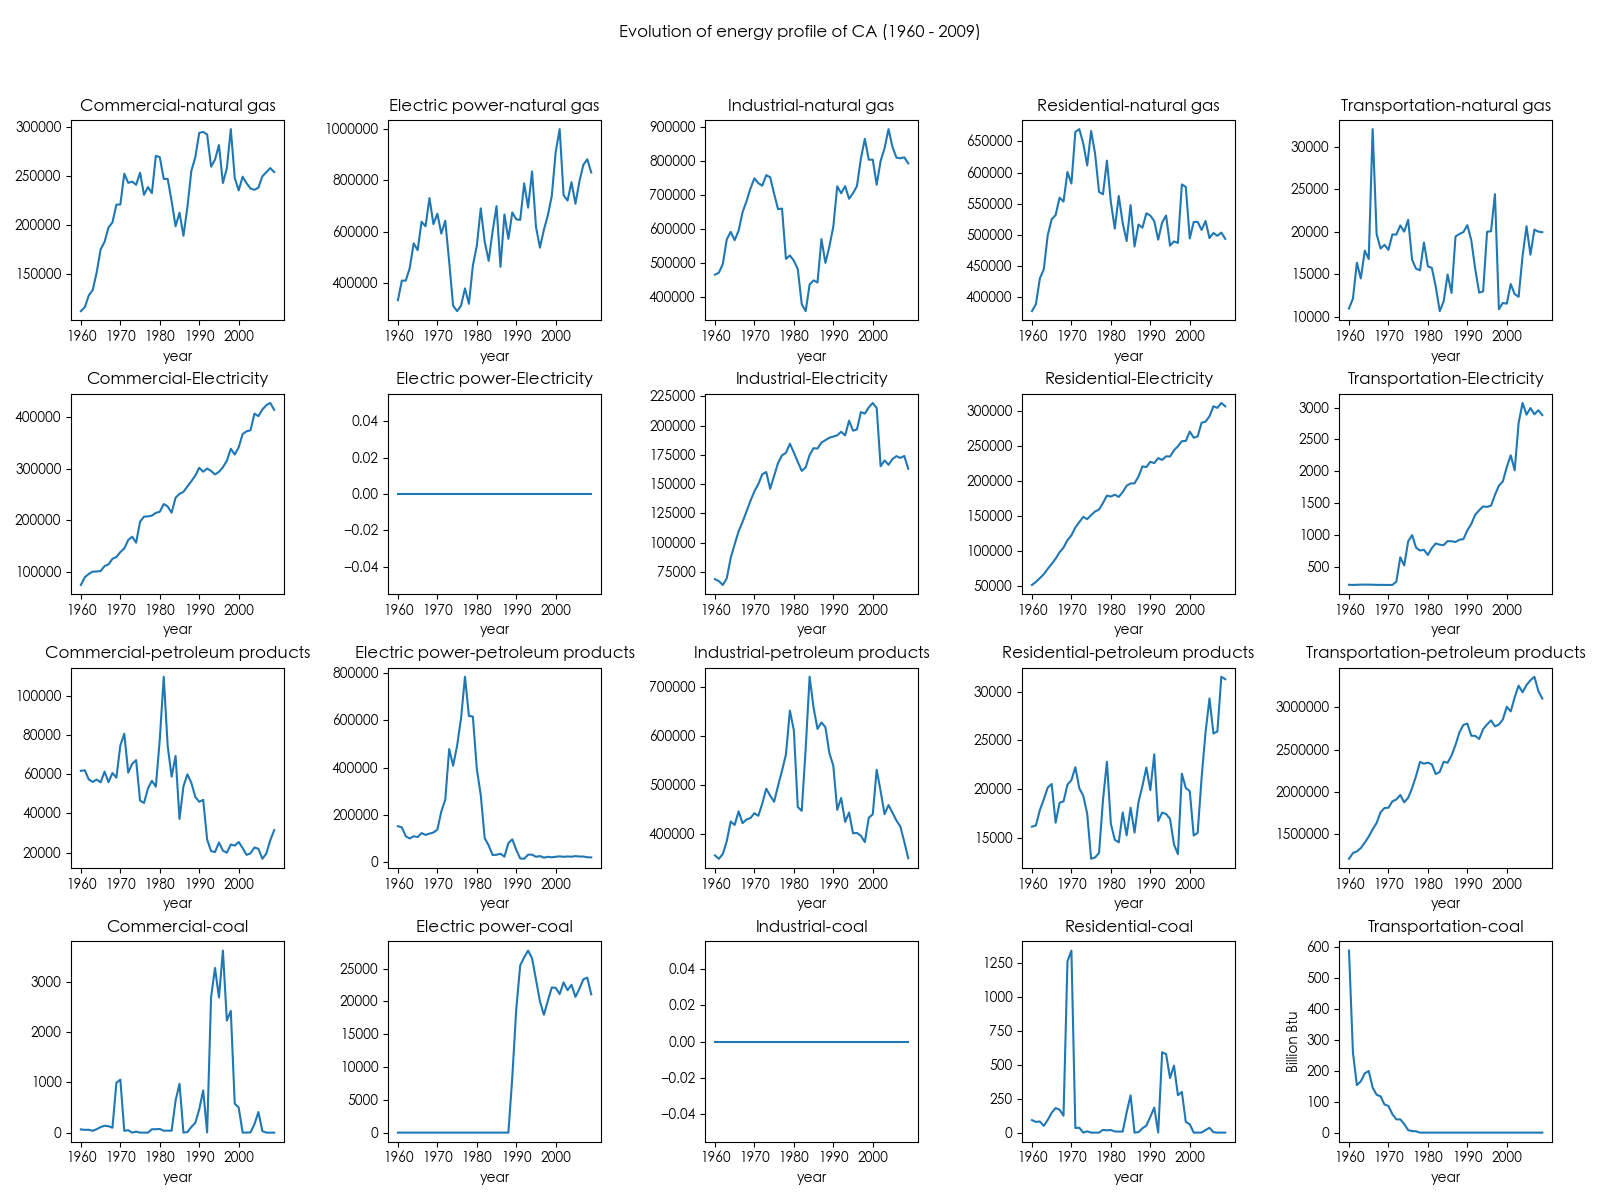
\includegraphics[width=0.85\textwidth]{./Pic/B-classify-CA.png}
    % 图片标题
    \caption{Evolution of energy profile of CA (1960-2009).}
    \label{fig:part-2-CA}  
\end{figure}

% 5.1.2
\subsubsection{Brief analysis of the evolution above}
\par There are indeed some advantages of this model evolution, which are as follows
\begin{itemize}
    \item Comparison between the different classification of energy is well organized and can be seen directly and clearly.
    \item Different sectors have different impacts on energy usage, and this model can show the difference obviously.
    \item It is intelligible to see the trend of the energy usage changes over time.
    \item We can easily get to the conclusion that some sharp changes in the line chart are possibly caused by policy reform.  
\end{itemize}
\par However, we have to say it is undeniable that this evolution model has its disadvantages, which are as follows
\begin{itemize}
    \item It is hard to compare the influence of different factors in different states in this model, in other words, we can not see the comprehensive effect of all the factors together in energy usage influence.
    \item Governors are more care about the interstate difference in energy usage, but this model is not intuitively enough.
    \item The model doesn't pay much attention to the usage of renewable energy, which is an important part of our problem.
\end{itemize}
\par In order to improve the shortcomings, we build a new model, named Analytic Hierarchy Process (AHP), to satisfy the demand of the governors.


% 5.2
\subsection{Energy Usage Comparison Model}

\par With analytic hierarchy process(AHP) model, we can obtain scores of the total renewable energy usage of the four states, through which we can analyze the similarities and differences between the four states. 
% TODO: 使用摘要中的语句
% 5.2.1
\subsubsection{Analytic hierarchy and factor origin}

\par The first step to build the model is to find key factors influencing the state comparison. There is no doubt that the target comparing object is the usage of renewable energy and the bottom layer is four states. Then we find that there are mainly five sectors in which all the energy be produced or consumed, so these sectors are the best factors to describe the influence of energy usage similarities and differences between the four states.

\par The five sectors are transportation, commerce, electricity, industry, and resident. Resident naturally represents population, and transportation is closely linked with geography \cite{L1}. So our factors contain some of the possible influential factors of the similarities and differences described in the question, but they are more detailed and energy-concerned.

\par After getting the comparison results of total renewable energy usage, we start to focus on the per capita renewable energy usage. It is reasonable that different population of a state results in different energy usage. So we divide the renewable energy usage of every sector by population and calculate its result of AHP.

% 5.2.2
\subsubsection{Establishment of AHP model}

\par For obtaining the renewable energy proportion of each sector, we need renewable energy total comsumption values of each sector which can be computed by formula in the MSN refercence:

\par We make Y be the usage level of renewable energy as the target, and $X_i$ represent the five sectors which means the standard of comparison. Therefore, we have the analytic hierarchy model based on total renewable energy usage as follows.\cite{6}

\begin{figure}[H] 
    \centering 
    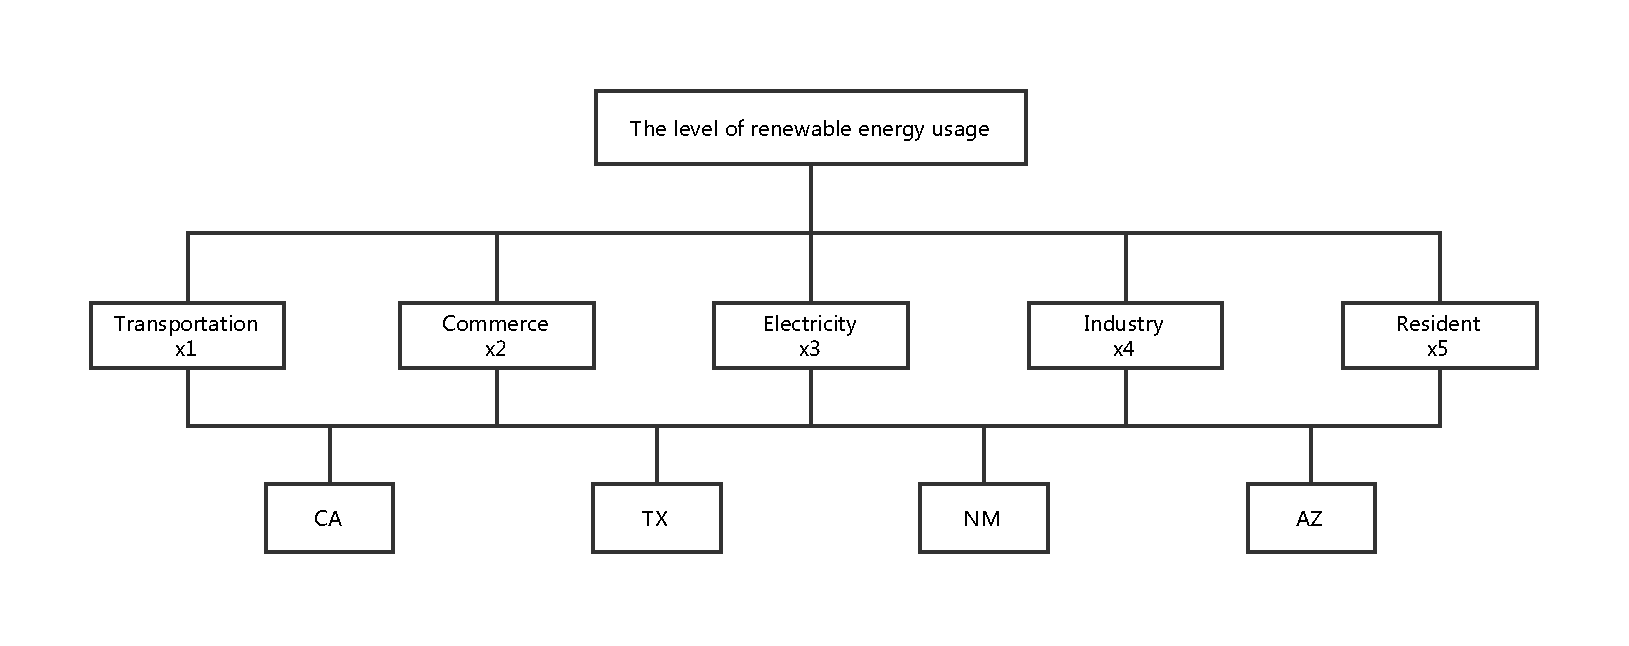
\includegraphics[width=0.8\textwidth]{./Pic/AHP.pdf}
    \caption{AHP model}
\end{figure}

\par In order to analyze the closeness between each of the sectors and Y, we analyze the given data to obtain the total renewable energy usage of each sector. According to the calculation method of the pairwise comparison matrix, we can obtain C, the pairwise comparison matrix of the five sectors under Y. We then calculate $\lambda_m$(C) , the maximum of the eigenvalues of C. Here, n is equal to 4 and RI is equal to 1.12.\cite{6} If C can not pass the check equation for consistency:
\begin{equation}
    \centering
    CI=\frac{ \lambda_m(C)-n }{ n-1 }
\end{equation}
\begin{equation}
        \centering
    CR=\frac{ CI }{ RI }<0.1 
\end{equation}

\par We will recalculate C until C pass the check of consistency. Then we calculate $\beta$, the eigenvector of $\lambda_m$(C), which must meet the conditions that the sum of the coordinates of the eigenvector is 1 and the coordinates are greater than 0, and we call it weight vector.
\par Similarly, we can also obtain $B_i$, the pairwise comparison matrix of the four states under $X_i$, and $\beta_i$, the weight vector of $X_i$.
\par We define U as follows: % TODO: follows?
\begin{equation}
    \centering
U=\begin{pmatrix} \beta_1 & \beta_2 & \beta_3 & \beta_4\end{pmatrix}
\end{equation}
\par Finally, we can obtain the scores based on the total energy usage of the four states:

\begin{equation}
    \label{AHP_result}
    \begin{array}{l}
    \displaystyle CA=\sum_{i=1}^{5}\beta[i] \times U[i,1] \\
    \displaystyle TX=\sum_{i=1}^{5}\beta[i] \times U[i,2] \\
    \displaystyle NM=\sum_{i=1}^{5}\beta[i] \times U[i,3] \\
    \displaystyle AZ=\sum_{i=1}^{5}\beta[i] \times U[i,4]
    \end{array}
\end{equation}

% 5.2.3
\subsubsection{Calculation results of AHP model}
\par Firstly, we can get the renewable energy comsumption of each sector by MSN formulas \cite{4} as following table:

\begin{table}[!hbp]
    \centering 
    \begin{tabular}{|c|c|}
    \hline Comsumption & MSNs \\
    \hline transportation & \text{EMACB} \\
    \hline commercial &  \text{EMCCB} + \text{GECCB} + \text{HYCCB} + \text{SOCCB} + \text{WWCCB} + \text{WYCCB} \\
    \hline electric power & \text{HYEGB} + \text{GEEGB} + \text{SOEGB} + \text{WWEIB} + \text{WYEGB} \\
    \hline industrial & \text{EMICB} + \text{EMLCB} + \text{GEICB} + \text{HYICB} + \text{SOICB} + \text{WWICB} + \text{WYICB} \\
    \hline residential & \text{WDRCB} + \text{GERCB} + \text{SORCB} \\
    \hline
    \end{tabular}
    \caption{The various sectors renewable energy consumption and MSN relationship table}
    \label{tab:sector-msn}
\end{table}

% \begin{align*}
%     & \text{transportation} = \text{EMACB} \\
%     & \text{commercial} = \text{EMCCB} + \text{GECCB} + \text{HYCCB} + \text{SOCCB} + \text{WWCCB} + \text{WYCCB} \\
%     & \text{electric power} = \text{HYEGB} + \text{GEEGB} + \text{SOEGB} + \text{WWEIB} + \text{WYEGB} \\
%     & \text{industrial} = \text{EMICB} + \text{EMLCB} + \text{GEICB} + \text{HYICB} + \text{SOICB} + \text{WWICB} + \text{WYICB} \\
%     & \text{residential} = \text{WDRCB} + \text{GERCB} + \text{SORCB} \\
% \end{align*}

\par Then, we divide the given data by year, and calculate the scores of the four states in 2009 as follows:
\[
    \text{CA}=55.6555729\%, \text{TX}=38.04528274\%, \text{NM}=0.997192757\%, \text{AZ}=5.301951596\%
\]
Clearly, the score of California and Texas is much greater than New Mexico and Arizona.
Then we calculate the scores of the four states in every year(1960 - 2009) and draw a line chart as follows.
\begin{figure}[!hptb] 
    \centering 
    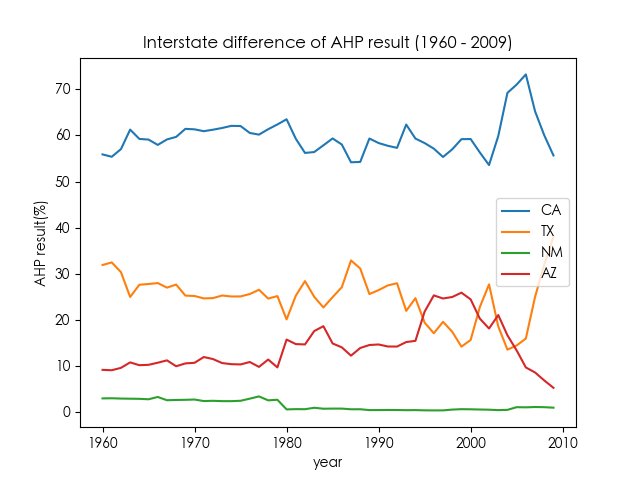
\includegraphics[width=0.7\textwidth]{./Pic/B-level-predict.png}
    \caption{Scores based on the total renewable energy usage from 1960 to 2009}
    \label{fig:B-level-predict}
\end{figure}

% 5.2.4
\subsubsection{Result of per capita usage}
\par In order to have a more detailed and more comprehensive comparison of the similarities and differences of the states, we hold the view that it is not enough to compare the proportion of the renewable energy usage among states, sector usage difference within the state is also an important comparing factor.
\par When we talk about the analytic hierarchy model based on per capita renewable energy usage, we just need to change the values of CA, TX, NM, AZ to the values of CA, TX, NM, AZ divided by the total population of each state. Therefore, similarly, we can obtain the scores based on the per capita energy usage of the four states in each year from 1960 to 2009, and draw the line chart as follows.
\begin{figure}[H] 
    \centering 
    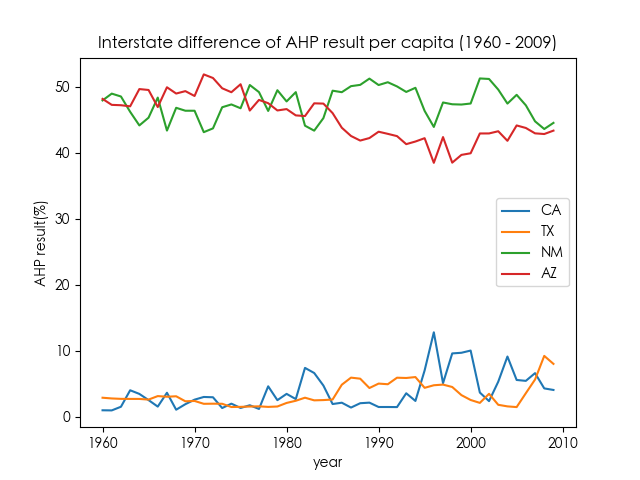
\includegraphics[width=0.7\textwidth]{./Pic/B-level-percapita.png}
    \caption{Scores based on the per capita renewable energy usage from 1960 to 2009}
    \label{fig:B-level-percapita}
\end{figure}

\subsection{Similarities and differences analysis}



\par We have taken the five sectors' influence into consideration in the AHP model to get the renewable energy usage proportion, and it works well when comparing the sector influence among four states, but it can not describe the proportion of different sectors in a state. So we calculate the proportion of renewable energy usage of different sectors in every state in every year from 1960 to 2009 and obtain figure \ref{fig:B-percent}.


\par We have to take the five sectors' influence into consideration in the AHP model to get the renewable energy usage proportion, and it works well when comparing the sector influence among four states, but it can not describe the proportion of different sectors in a state. So we calculate the proportion of renewable energy usage of different sectors in every state in every year from 1960 to 2009 and get figure \ref{fig:B-percent}. According to figure \ref{fig:B-level-predict} and figure \ref{fig:B-percent} we can conclude the similarities and differences.

\begin{figure}[H]%[!hptb] 
    \centering 
    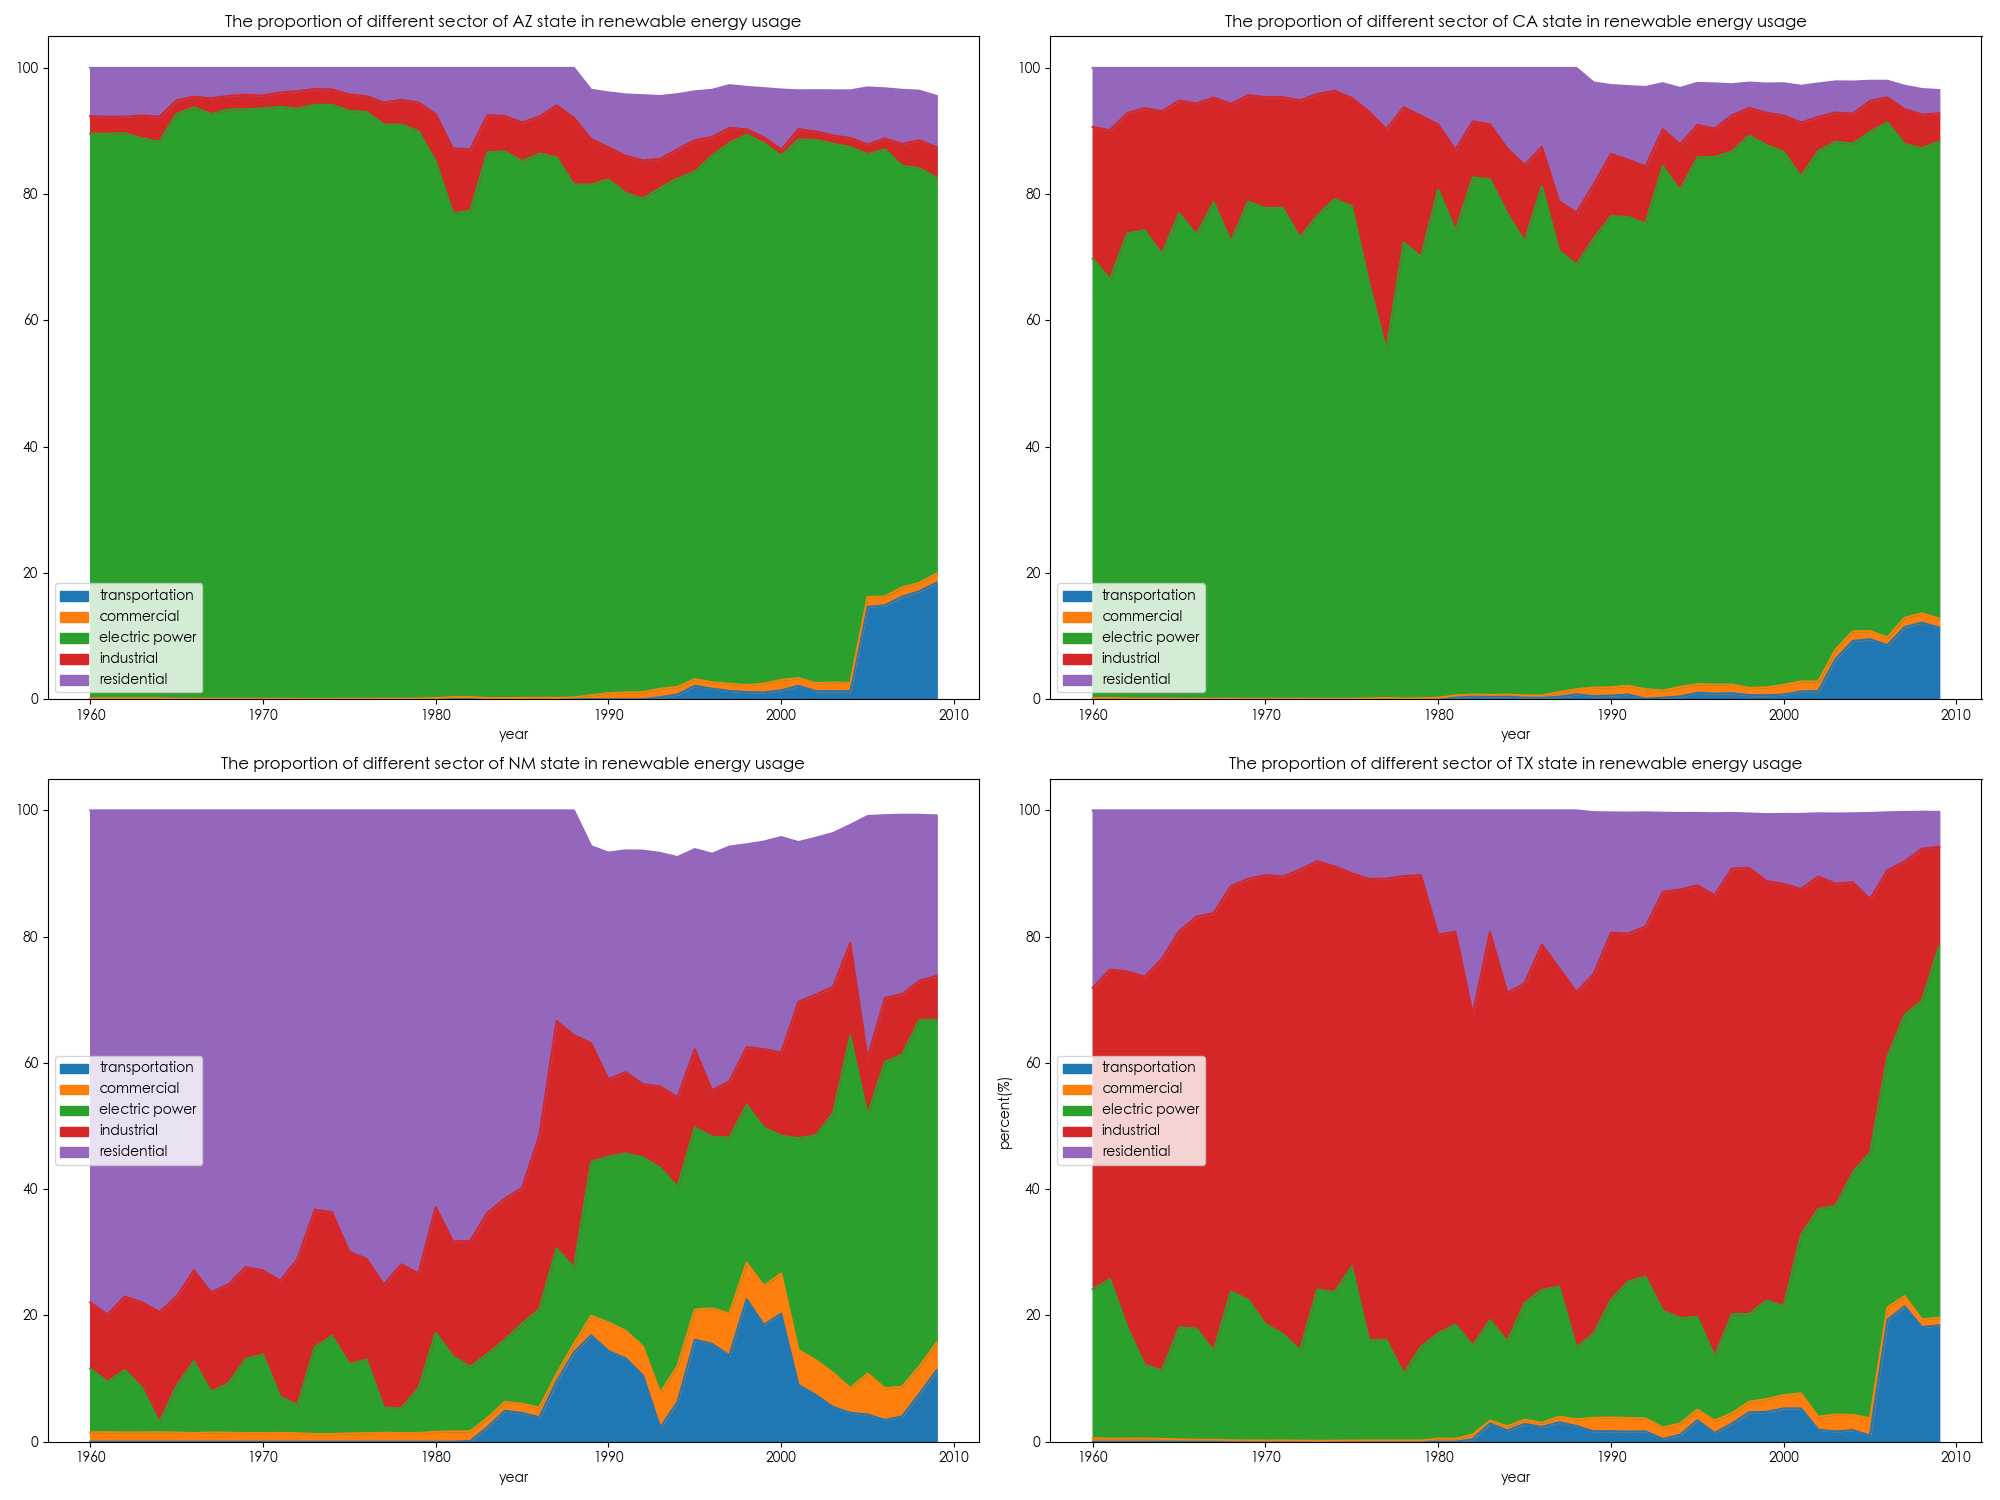
\includegraphics[width=1\textwidth]{./Pic/B-percent.png}
    % 图片标题
    \caption{The proportion of renewable energy usage of different sectors of four states in 2009}
    \label{fig:B-percent}  
\end{figure}

% TODO: which diffs?

% 5.3.1
\subsubsection{Differences among the four states}

\begin{itemize}
    \item Different states account for a different proportion of the total renewable energy usage. California always accounts for the most while New Mexico always accounts for the least.
    \item Different states have a different level of the p capita renewable energy usage. California and Texas always account for the least while New Mexico and Arizona always account for the most.
    \item The fluctuation of the proportion of New Mexico is not so obvious, but other three states have changed a lot.
    \item After 2000, the score based on the total renewable energy of Arizona has a steady trend of declining, while other states keep fluctuating.
    \item Different state has different major usage of renewable energy. California and Arizona use renewable energy mainly in electric power, New Mexico mainly in resident sector and Texas mainly in industry.
    \item The distribution of total renewable energy usage has changed a lot in all of the four states, but the changing trend of each state is different from others.
    
\end{itemize}

% 5.3.2
\subsubsection{Similarities among the four states}

\begin{itemize}
    \item All of the states can be easily affected by the policy change, which can be inferred from the sharp rise and fall in the figure.
    \item All of the states have a different distribution of total renewable energy usage.
    \item All of the states have little renewable energy usage in the commercial sector.
    \item All of the states have a trend of increasing proportion of transportation, while it was almost zero at first.
    \item All of the states do not have a huge change in the level of per capita renewable energy usage from 1960 to 2009.
\end{itemize}


% 6
\section{Best Profile Analysis Model}

\par The governors are interested in forming a realistic new energy compact focused on increased usage of cleaner, renewable energy sources. But before building the compact, it is of great significance to compare the renewable energy use profile among four states and get the best profile to encourage states to accelerate the development of renewable energy.

\par We have compared the profile of four states in the previous section a lot, so in this part, we focus on setting up a series of criteria and choosing the best profile of them. 

\subsection{Model Construction}
\par Let $\phi_i$ represents the proportion of each state , $\Phi_i$ represents the per capita renewable energy usage proportion of each state in 2009, then the biggest value of them can be described as

\begin{equation}
    \phi_{max} = MAX({\phi_i|i=1,2,3,4})
\end{equation}
\begin{equation}
    \Phi_{max} = MAX({\Phi_i|i=1,2,3,4})
\end{equation}

\par Let $\kappa_i$ be the gradient of every state, then 

\begin{equation}
    \kappa = \frac{\Delta \phi_i}{\Delta year}
\end{equation}
\begin{equation}
    \kappa_{max} = MAX({\kappa_i | i=1,2,3,4})
\end{equation}

\par Let $\mu_i$ be the gradient of every state, then 
\begin{equation}
    \mu = \frac{\Delta \Phi_i}{\Delta year}
\end{equation}
\begin{equation}
    \mu_{max} = MAX({\mu_i | i=1,2,3,4})
\end{equation}

\subsection{Best profile in renewable energy usage amount}

\par Based on the result of Problem B, we can get the scores of the importance of renewable energy usage of different states, which actually stands for the state's proportion of renewable energy usage in all states under the influence of five sectors. On this occasion, we can get the biggest proportion, which represents the state that uses the most renewable energy in the year. We can get the result as follows from the calculation of Problem B

\begin{equation}
    \phi_{1} = 55.65557290,~~ \phi_{2} = 38.04528274,~~ \phi_{3} = 0.99719276,~~ \phi_{4} = 5.30195160
\end{equation}

\par $\phi_{max} = \phi_{1}$, so the biggest proportion is $\phi_{1}$, which means that \textbf{California} has the biggest energy usage amount in 2009.

\par But other governors may have different opinions, they may hold the view that it is unfair since California has the biggest population. On this occasion, we will take the result of per capita usage for analysis. Then we can get the data

\begin{equation}
    \Phi_{1} = 4.05334714,~~ \Phi_{2} = 8.00804230,~~ \Phi_{3} = 44.55708957,~~ \Phi_{4} = 43.38152098
\end{equation}
\par $\Phi_{max} = \Phi_{3}$, so the biggest per capita proportion is $\Phi_{3}$, which means that \textbf{New Mexico} has the biggest per capita energy usage amount in 2009.

\subsection{Best profile in increase of renewable energy usage}

\par Besides total amount of renewable energy usage, we think that it is also indispensable to take usage increase rate into consideration, because increase rate can reflect a state's growing concern about the renewable energy and can represent the progress in renewable energy usage. It is also an important factor when judging the "best" profile.

\par The best description of the increase of renewable energy usage is its gradient in the line chart. So we take $\kappa$ into consideration and bring data into the formula, then we get results
\begin{equation}
    \kappa_{1} = -4.36938978,~~ \kappa_{2} = 6.07795471,~~ \kappa_{3} = -0.10693533,~~ \kappa_{4} = -1.60162960
\end{equation}
\par $\kappa_{max} = \kappa_{2}$, so \textbf{Texas} has the biggest increase rate in 2009.

\par Similarly, we take population into consideration and get the gradient of the  proportion of per capita renewable energy usage. 

\par Then we bring data into the formula and get results
\begin{equation}
    \mu_{1} = -0.23615508,~~ \mu_{2} = -1.21046745,~~ \mu_{3} = 0.93103726,~~ \mu_{4} = 0.51558527
\end{equation}
\par $\mu_{max} = \mu_{3}$, so \textbf{New Mexico} has the biggest per capita increase rate in 2009.

\subsection{Best profile choice}
\par In summary, there are a variety of perspectives to choose the best profile among the four state. Different states have their own best performance in different perspectives, but after taking various factors into consideration,  \textbf{New Mexico} has the best performance in renewable energy usage.
So the best profile of 2009 belongs to \textbf{New Mexico}.

% \subsection{The reasons for not considering economic factors}
% \par Some people may think that economy is an essential factor when choosing the best profile. However, after analysis, we are able to prove that economic fatcors do not need to be considered.
% \par It is 

% Chapter 7
\section{Prediction Model}
\par Based on the results of problem B, we build regression equations, which show the relationships between the scores of the four states and years, so that we can predict the scores of the four states in 2025 and 2050.
\subsection{Regression analysis model}  
\subsubsection{Establishment of regression equations}
\par In problem D, the policy about the energy of each state will not change until 2050. At first, we consider the levels of the total renewable energy usage of the four states.  According to Figure \ref{fig:B-level-predict}, from 1995 to 2009, the scores of New Mexico and Arizona have a consistent trend, we consider it as the absence of any policy change. Meanwhile, for California and Texas, their scores have a sudden change after 2005, we consider it is because of policy change. Therefore, we use the scores of New Mexico and Arizona from 1995 to 2009, and the scores of California and Texas from 2005 to 2009 to build the regression equations.
\par For California and Arizona, we use exponential function to fit curves. And for New Mexico, we use linear regression.
\par We suppose the linear regression equation is
\begin{equation}
    \centering
\text   y=ax+b
\end{equation}
and we have ($x_i$, $y_i$), i=1 to n, which is paired data of x and y. By generalized least squares, we can obtain the value of a and b.
\par When we want to obtain fitted curve by exponential function, we suppose the regression equation is
\begin{equation}
    \centering
\text   y=be^{ax}
\end{equation}
The equation is equal to
\begin{equation}
    \centering
\text   log(y)=log(b)+ax
\end{equation}
which is a linear regression equation, so that we can use generalized least squares to calculate the value of a and b.

\subsubsection{Results of Regressions}
\par The regression equations are
\begin{equation}
    \centering
\text{CA}:   Z_1=e^{-0.34649 \times year+697.98712}+50
\end{equation}
\begin{equation}
    \centering
\text{TX}:   Z_2=100-CA-NM-AZ
\end{equation}
\begin{equation}
    \centering
\text{NM}:   Z_3=0.05263 \times year-104.64807
\end{equation}
\begin{equation}
    \centering
\text{AZ}:   Z_4=e^{-0.10513 \times year+213.24602}
\end{equation}
\par The Pr of F-test and t-test are all less than 0.05. Therefore, according to assumption 2, all of the regressions are effective and the independences between the parameters are very good.
\par The $R^{2}$ of each regression are greater than 0.68, even over 0.8. Therefore, according to assumption 3, all of the effects of the regressions are good.
\par In order to obtain S, which is the amount of the total renewable energy usage of each state in future, we need to predict the total renewable energy usage of the four states.
\par According to Figure \ref{fig:D-total-energy} as follows,
\begin{figure}[h]%[!hptb] 
    \centering 
    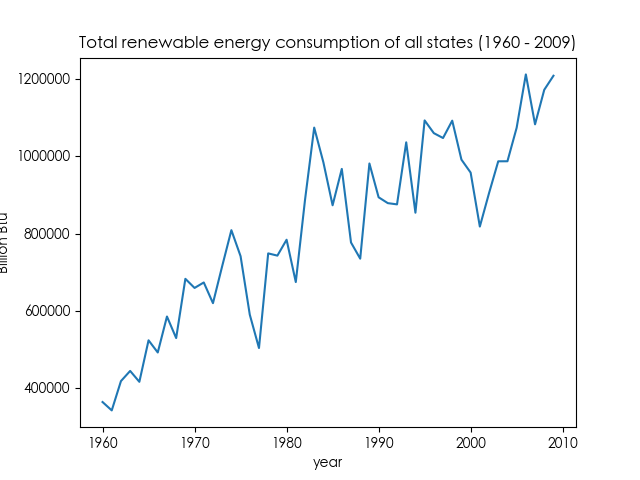
\includegraphics[width=0.7\textwidth]{./Pic/D-total-energy.png}
    \caption{Total renewable energy usage of the four states from 1960 to 2009}
    \label{fig:D-total-energy}  
\end{figure}
we can find that we should bulid linear regression equation.
\begin{equation}
    \centering
S=14466 \times year-27896894
\end{equation}
\par Amount of the renewable energy usage of each state in every year is:
\begin{equation}
    \centering
    S_i=0.01 \times S \times Z_i
\end{equation}

\subsubsection{Scores of the four states in future}
\par According to the regression equations, we can obtain the score based on the total renewable energy usage and amount of the total renewable energy usage of each state in 2025 and 2050 as follows.
\begin{table}[!hbp]
    \centering 
    \begin{tabular}{|c|c|c|c|c|}
\hline
State & Score-Total in 2025 & Amount in 2025 & Score-Total in 2050 & Amount in 2050\\
\hline
California & 50.04186\% & 698962.6821 & 50.00001\% & 879203.1758 \\
\hline
Texas & 46.76163\% & 653145.8727 & 47.29053\% & 831559.5170 \\
\hline
New Mexico & 1.59588\% & 222290.54965 & 2.56588\% & 45118.58787 \\
\hline
Arizona & 1.60063\% & 22356.89556 & 0.14358\% &2524.719335 \\
\hline
Total amount & 100\% & 1396756 & 100\% & 1758406 \\
\hline
\end{tabular}
\caption{Scores and amounts of four states in 2025 and 2050}
\label{tab:Scores and amounts}
\end{table}
\par Besides, we draw the graph of the regression equations as follows.
\begin{figure}[h]%[!hptb] 
    \centering 
    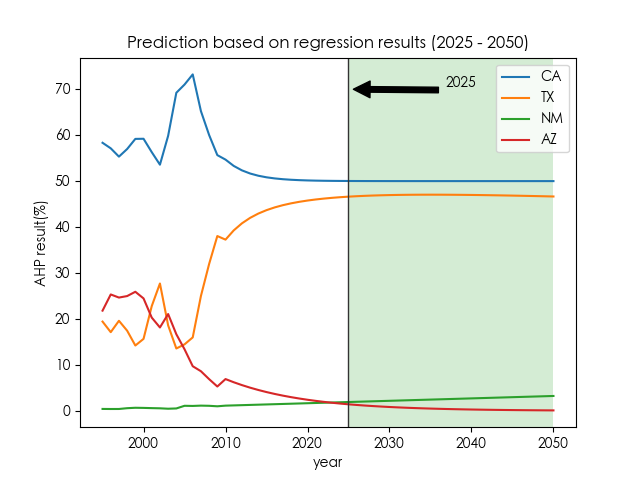
\includegraphics[width=0.7\textwidth]{./Pic/D-scores.png}
    \caption{Scores based on total renewable energy of the four states from 1960 to 2050}
    \label{fig:D-scores}  
\end{figure}
\par Besides, we also need to consider the levels of per capita renewable energy usage of the four states. According to figure \ref{fig:B-level-percapita}, we can find that each score based on per capita renewable energy usage is in a approximate region.
\[
CA:[1,10], TX:[1,10], NM:[43,50], AZ:[40,50]
\]

\subsection{Analysis of the results}
\subsubsection{Level and amount of total renewable energy usage}
\par From 2025 to 2050, based on the total renewable energy usage, score of California is very close to 50.00000 and continues to decline, score of Arizona will begin to be less than the score of New Mexico and will be close to 0 in 2050. On the contrary, score of Texas keeps growing but is not greater than the score of California, and the score of New Mexico grows at a slow rate.
\par Therefore, comparing to other states, the levels and amounts of total renewable energy usage of the four states are as follows.
\begin{itemize}
    \item California: level declines but still is the best, meanwhile, amount keeps growing.
    \item Texas: both of level and amount keep growing and gets close to California.
    \item New Mexico: both of level and amount get better than Arizona and also keep growing.
    \item Arizona: both of level and amount keep declining.
\end{itemize}
\subsubsection{Level of pre capita renewable energy usage}
\par The scores based on the per capita renewable energy usage do not have a huge change, they will be still in the region in 2025 and 2050.
\par Therefore, comparing to other states, the level of per capita renewable energy usage are as follows.
\begin{itemize}
    \item California and Texas: are still the lowest.
    \item New Mexico and Arizona: are still the highest.
\end{itemize}












\section{Renewable energy usage targets for 2025 and 2050}
\par According to the results of Problem D, we have predicted the amounts of total renewable energy when the policy dose not change. Therefore, we can build target model, which can give renewable energy usage targets for the four states in 2025 and 2050.
\subsection{Target model}
\par For California, Texas, and New Mexico in any year, we define the target is the predicted value of the amount of total renewable energy because the amounts of the total renewable energy usage of them keep growing.
\par For Arizona, its predicted value of the amount of total renewable energy keeps declining and will get less than New Mexico. Therefore, we define the target is
\begin{equation}
    \centering
    Target=0.01*(5.30195+0.05263 \times (year-2009))*S
\end{equation}
which means from 2009, the score based on the total energy usage keep growing at the same rate of New Mexico.
\par If the real amount of the total renewable energy usage is not less than the predicted value of amount of the total renewable energy, we consider it as the goal of the new four-state energy compact.
\subsection{Results of target model in 2025 and 2050}
\par According to table \ref{tab:Scores and amounts} and the target model, we have the target of each state in 2025 and 2050 as follows.
\begin{table}[H]
    \centering 
    \begin{tabular}{|c|c|c|}
\hline
State & Target in 2025 (Billion Btu) & Target in 2050 (Billion Btu)\\
\hline
California & 698962.6821 & 879203.1758 \\
\hline
Texas & 653145.8727 & 831559.5170 \\
\hline
New Mexico & 22290.54965 & 45118.58787 \\
\hline
Arizona & 85817.10767 & 130949.4257 \\
\hline
\end{tabular}
\caption{Targets of the four states in 2025 and 2050}
\end{table}


\section{Actions for meeting goal}
\par In order to meet the goals above, the four states need to take some actions, especially Arizona. Here, we list four actions.
\begin{itemize}
    \item Increase the economic input to exploit technology for renewable energy. 
    \item Strengthen people's awareness of using renewable energy.
    \item Establish more renewable energy facilities, such as wind power plants and solar power plants to make more use of renewable energy.
    \item In the premise of no influence with the overall economy, limit the usage of non-renewable energy.
\end{itemize}

    



    




\section{Strengths and Weaknesses}

\paragraph{Strengths}
\text{\\}
\begin{enumerate}%[(1)]
\renewcommand{\labelenumi}{(\theenumi)}
    \item We used factor analysis to obtain the energy profile of the four kinds of energy, besides the energy profile of renewable energy.
    \item We considered the influence of the total population of each state, which made our model base on the situation of each state fully.
    \item Our models are effective when we deal with the data of other states or countries.
\end{enumerate}


\paragraph{Weaknesses}
\begin{enumerate}%[(1)]
\renewcommand{\labelenumi}{(\theenumi)}
    \item In factor analysis, we supposed that the corresponding valuables as the main factors when the cumulative percentage is over 0.65, it may not enough.
    \item Due to the amount of the data of scores is not enough, so that the results of regressions may not match future very much.
\end{enumerate}



\includepdf[pages=-]{memo.pdf}

% \newpage%另起一页书写正文

% \thispagestyle{empty}%本页不遍页码
%以下是参考文献
\phantomsection%生成该页的链接
\addcontentsline{toc}{section}{\refname}
\begin{thebibliography}{}

% 使用指令\bibitem 构造一条参考文献.
% 具体构造方式,参考以下参考文献格式说明以及示例
% 应尽可能使用英文格式
%
\bibitem{1}
Wikipedia, Interstate compact. \url{https://en.wikipedia.org/wiki/Interstate_compact}. 2018

\bibitem{2}
Gorsuch, R. L. Factor Analysis, 2nd edition. Hillsdale, NJ: Erlbaum. 1983

\bibitem{3}
U.S. Energy Information Administration, State Energy Data System (SEDS): 1960-2015 (complete). \url{https://www.eia.gov/state/seds/seds-data-complete.php}. 2017

\bibitem{4}
U.S. Energy Information Administration, State Energy Data System (SEDS): 1960-2015 (complete). \url{https://www.eia.gov/state/seds/sep_use/notes/use_a.pdf}. 2017.

\bibitem{5}
Tang Mengling, Wang zhanling, and Li Zhijian. Using Model of Factor Analysis to Calculate Weight and to Evaluate Water Quality[J]. Xingtai Vocational and Technical College, 2005.

\bibitem{RC}
U.S. Energy Information Administration, Renewable Energy Explained. \url{https://www.eia.gov/energyexplained/?page=renewable_home}. 2017


\bibitem{6}
Thomas L. Satty. How to make a decision: The Analytic Hierarchy Process[J]. University of Pittsburgh, 1990.

\bibitem{L1}
Jean-Paul Rodrigue, Claude Comtois, Brian Slack. Routledge, The Geography of Transport Systems. 2009.

\bibitem{7}
U.S. Energy Information Administration, State Energy Data System (SEDS): 1960-2015 (complete). \url{https://www.eia.gov/state/seds/sep_use/notes/use_c.pdf}. 2017


% etc
\end{thebibliography}


\newpage%另起一页书写
\begin{appendices} 
    % \pagestyle{empty}
    \section*{Figures}
\begin{figure}[h]%[!hptb] 
    \centering
    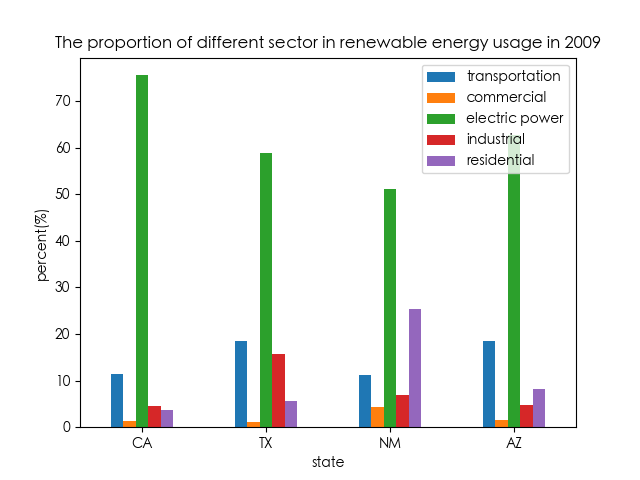
\includegraphics[width=0.7\textwidth]{./Pic/1-3.png}
    % 图片标题
    \caption{The weights of variables of the four states in 2009.}
\end{figure}
\begin{figure}[h]%[!hptb] 
    \centering
    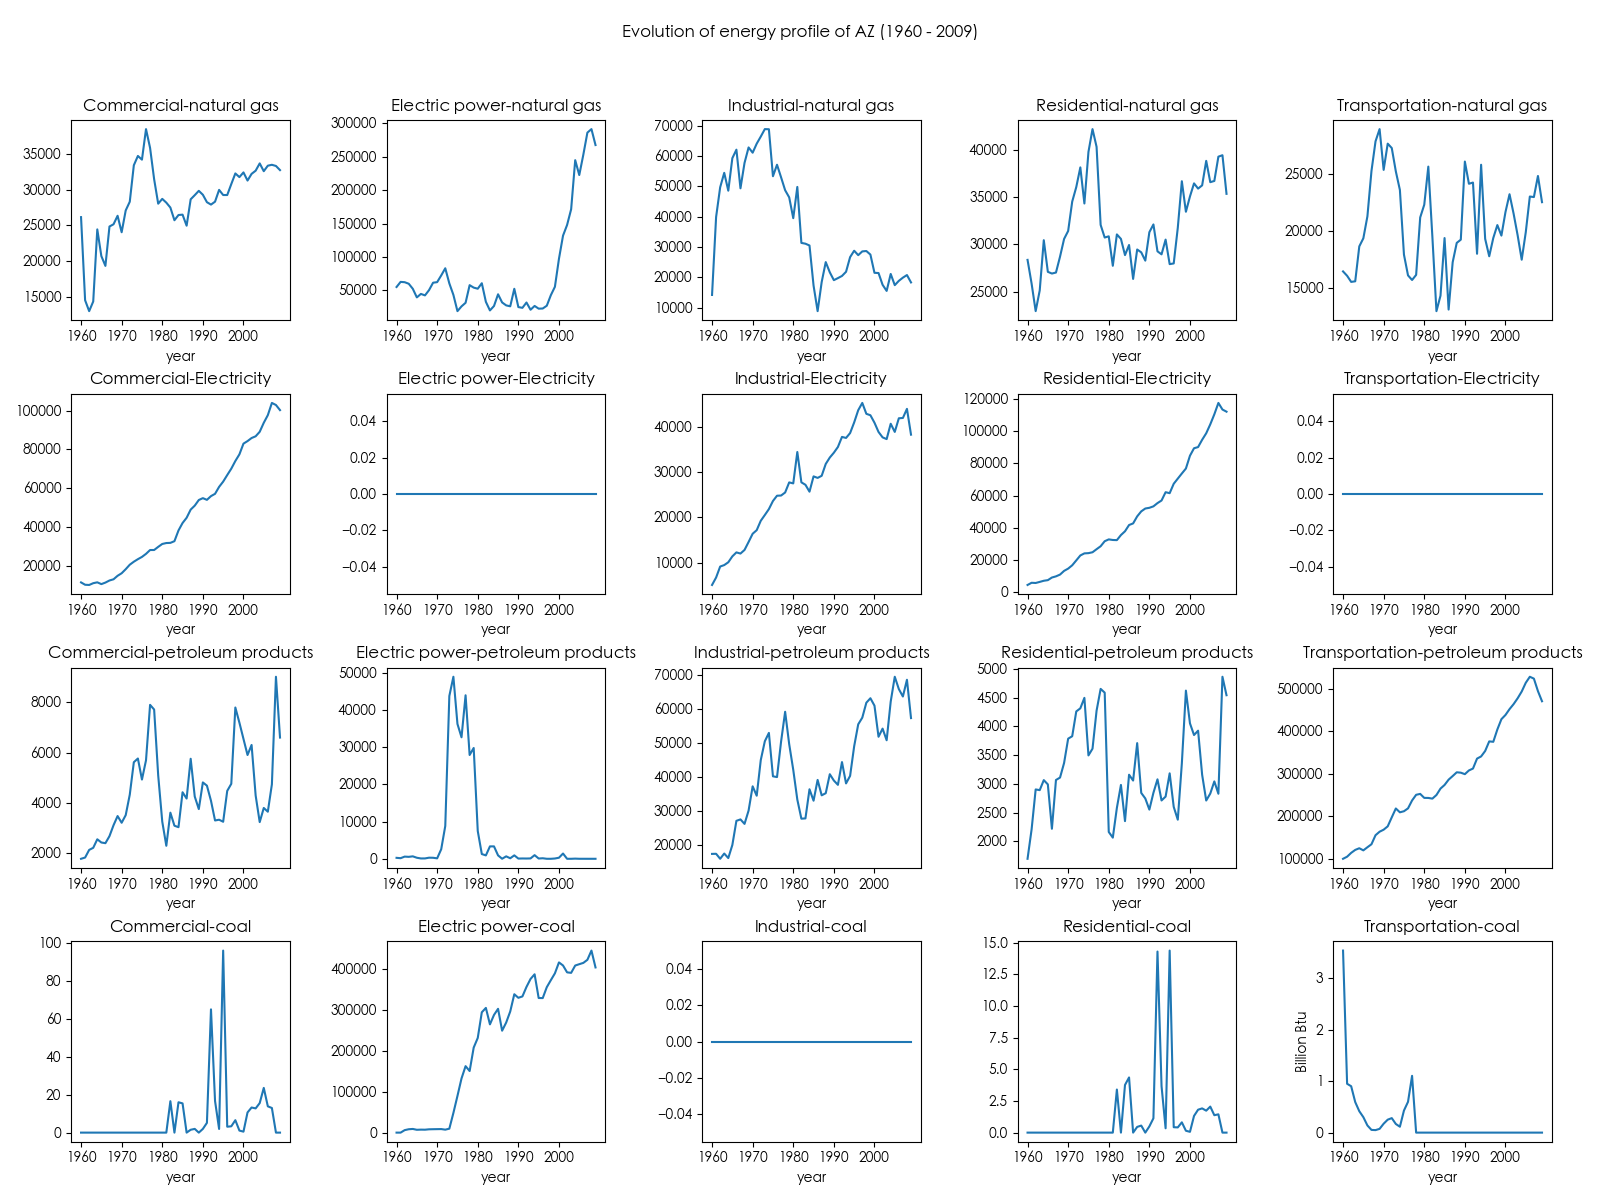
\includegraphics[width=0.7\textwidth]{./Pic/B-classify-AZ.png}
    % 图片标题
    \caption{Evolution of energy profile of AZ (1960-2009).}
    \label{fig:part-2-AZ}
\end{figure}

\begin{figure}[h]%[!hptb] 
    \centering 
    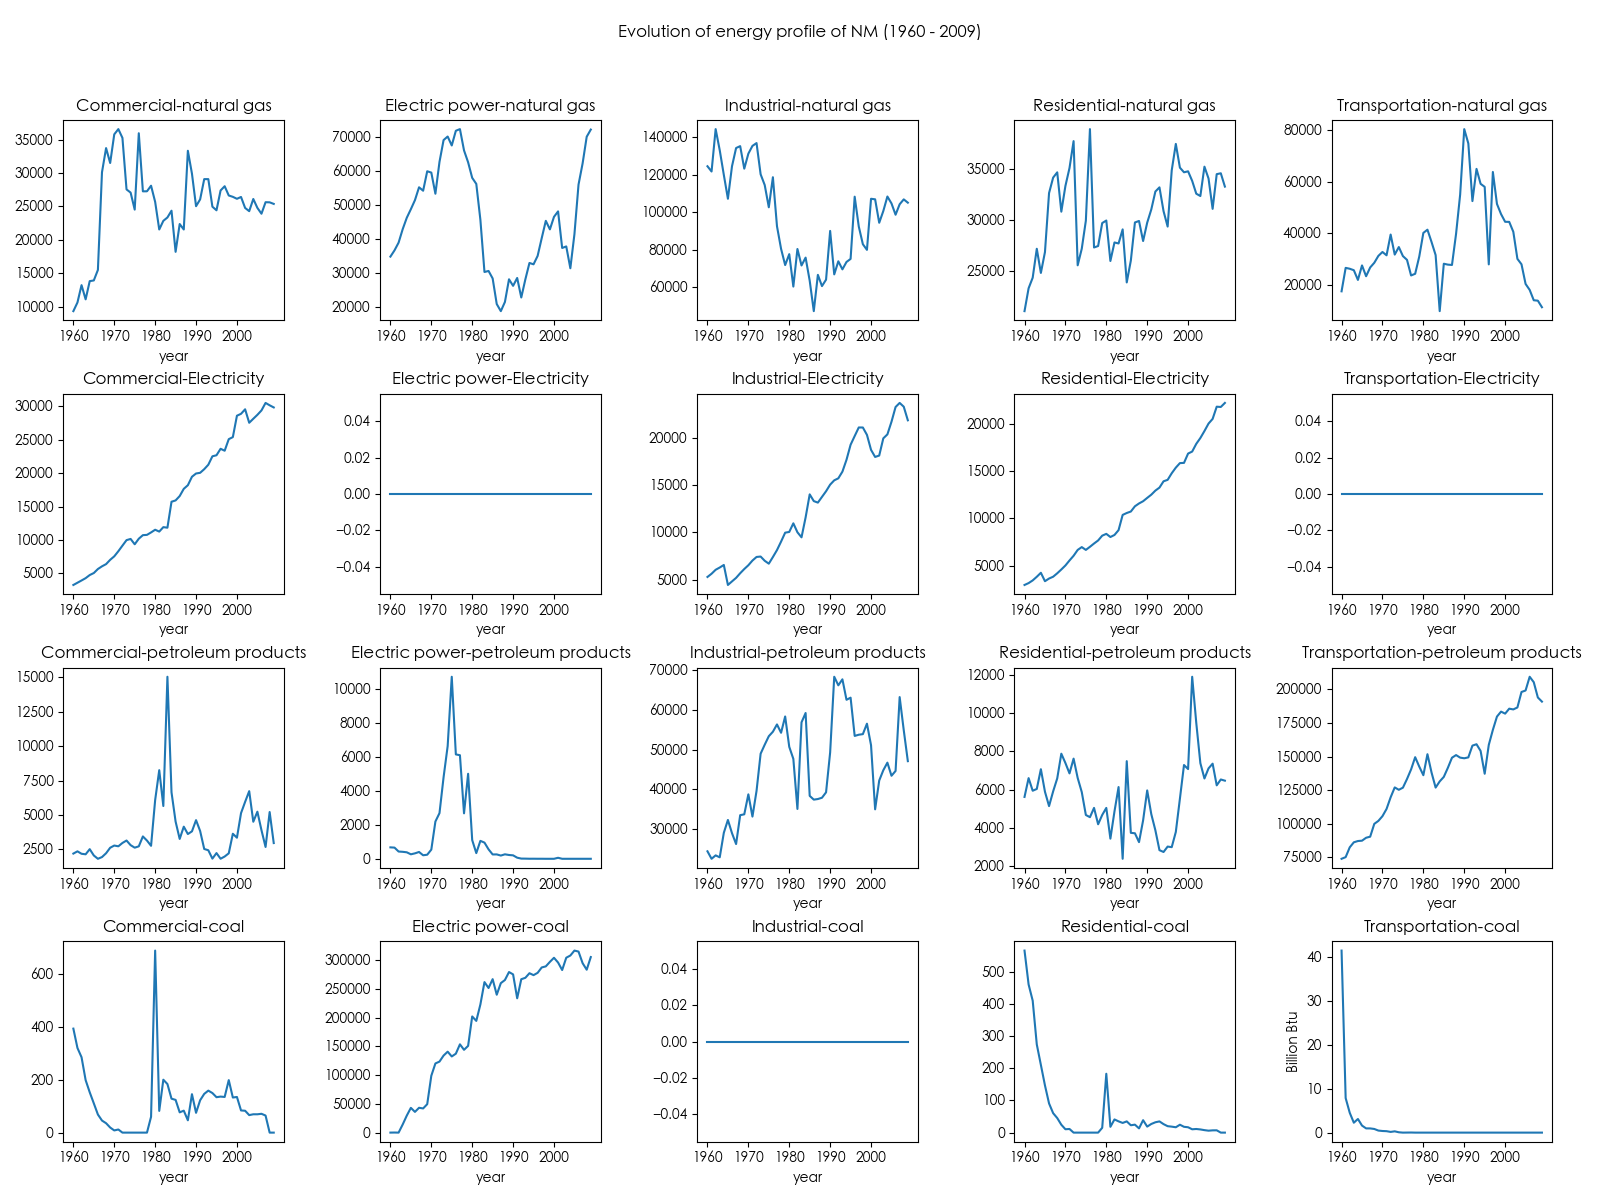
\includegraphics[width=0.7\textwidth]{./Pic/B-classify-NM.png}
    % 图片标题
    \caption{Evolution of energy profile of NM (1960-2009).}
    \label{fig:part-2-NM}  
\end{figure}

\begin{figure}[h]%[!hptb] 
    \centering 
    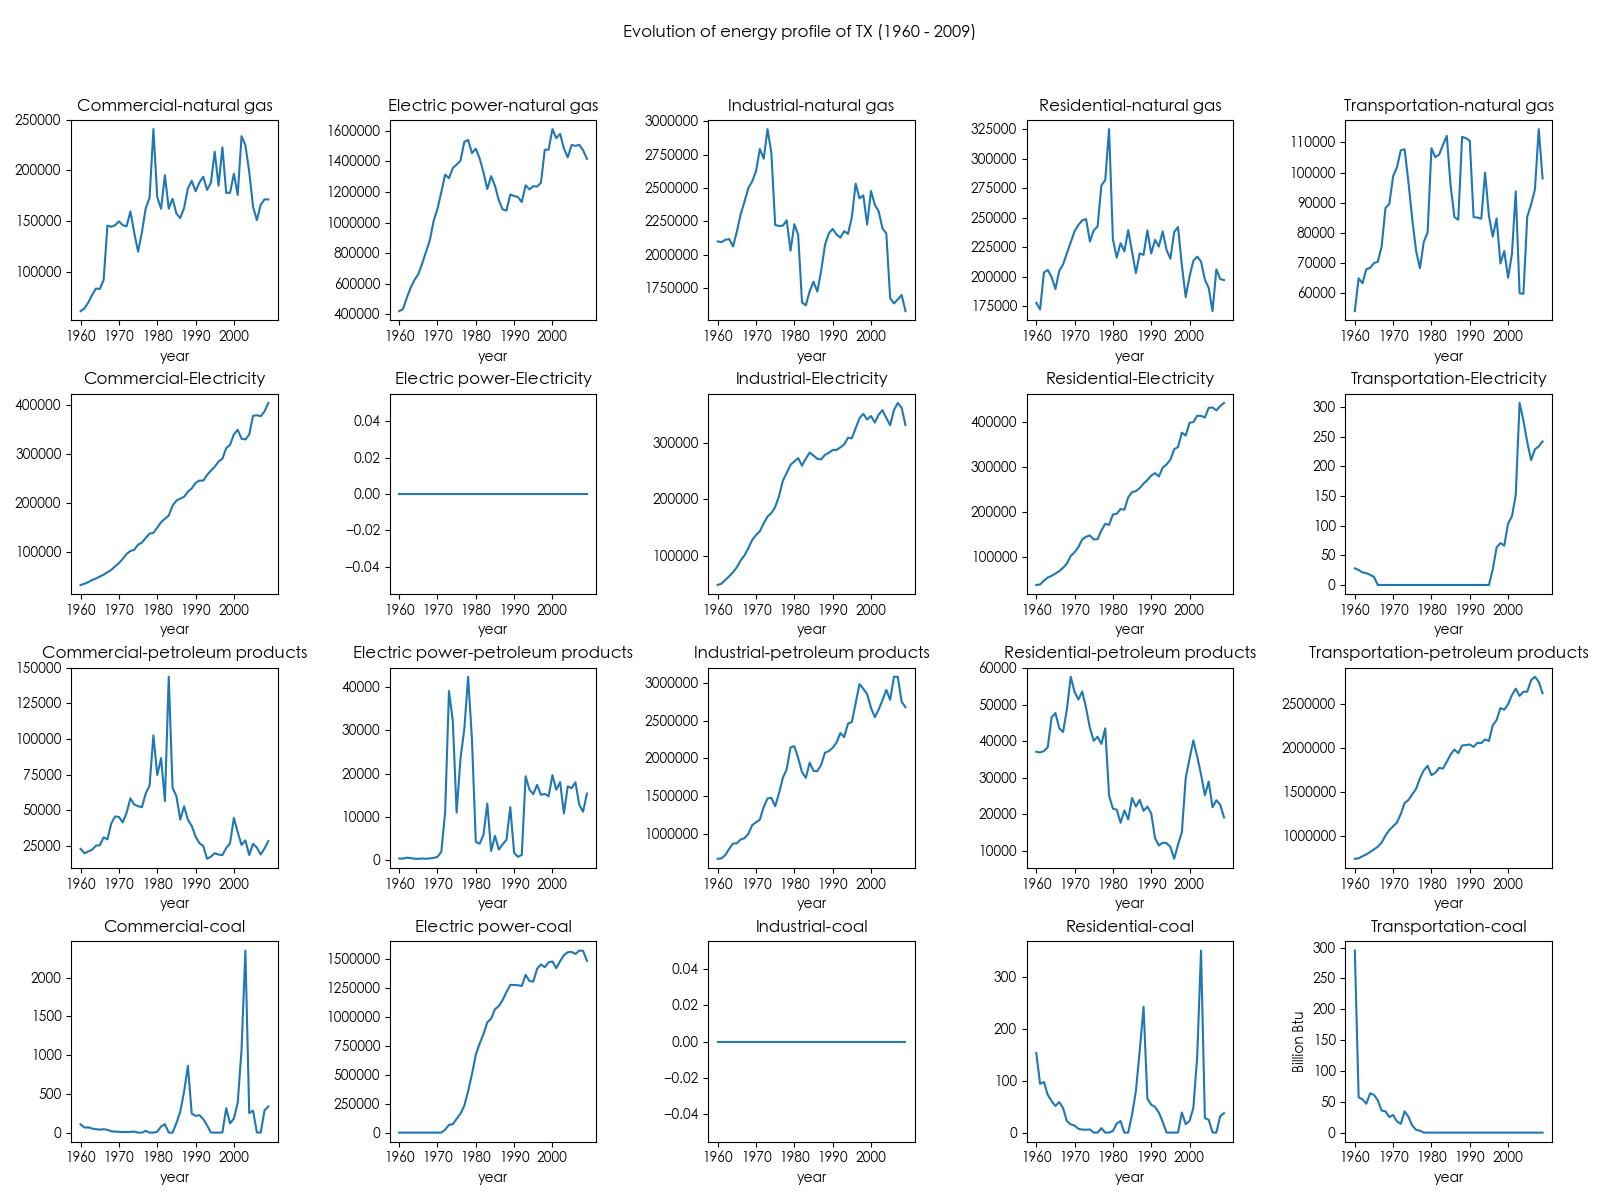
\includegraphics[width=0.7\textwidth]{./Pic/B-classify-TX.png}
    % 图片标题
    \caption{Evolution of energy profile of TX (1960-2009).}
    \label{fig:part-2-TX}  
\end{figure}
\section*{Codes}

\begin{lstlisting}[language=SAS, caption=regression.sas]
    data score1;
    set score;
    AZ1=log(AZ);
    CA1=log(CA-50);
    run;
    data score2;
    set score1;
    if year>=2005;
    run;
    proc reg data=score1;
    model NM=year;
    model AZ1=year;
    run;
    proc reg data=score2;
    model CA1=year;
    run;
    proc reg data=total;
    model total_renewable=year;
    run;
\end{lstlisting}

\begin{lstlisting}[language=Python, caption=score.py]

    def judge(a, b):
    x = [a, b] if a > b else [b, a]
    if x[1] == 0:
        x[1] = 0.000000001
    c = x[0] / x[1]
    p = 0
    if 1 < c <= 2.5:
        p = 2
    elif 2.5 < c <= 4.5:
        p = 3
    elif 4.5 < c <= 6:
        p = 4
    elif 6 < c <= 8:
        p = 5
    elif 8 < c <= 9.5:
        p = 6
    elif 9.5 < c <= 11.5:
        p = 7
    elif 11.5 < c <= 13:
        p = 8
    elif c == 1:
        p = 1
    else:
        p = 9
    return p if a > b else 1 / p


def get_matrix(l):
    matrix = [([1] * len(l)) for i in range(len(l))]
    for i in range(len(l)):
        for j in range(i, len(l)):
            matrix[i][j] = judge(l[i], l[j])
            matrix[j][i] = 1 / matrix[i][j]
    return matrix


def create_scores(years, filename, df_data, df_people=None):
    sectors = [msn for msn in SECTOR_MSN]
    df_score = pd.DataFrame(columns=['year'] + STATES)
    for year in years:
        df = create_clean_sector(year, df_data, True)
        clean_sectors_l = list(df[sectors].sum() / df['total'].sum() * 100)
        clean_sectors_matrix = get_matrix(clean_sectors_l)
        states_sectors_matrix = {}


        for sector in sectors:
            if df_people is not None:
                df = df[sectors].divide(df_people[str(year)], axis=0)
            sp = list(df[sector])
            states_sectors_matrix[sector] = get_matrix(sp)

        # lorry_cost = {'CA': 50000, 'TX': 25000, 'NM': 5000, 'AZ': 15000}
        criteria = sectors
        criteria_scores = clean_sectors_matrix

        options = STATES
        option_scores = states_sectors_matrix
        lorry_decision = analytical_hierarchy_process(criteria=tuple(criteria),
                                                        criteria_scores=criteria_scores,
                                                        options=tuple(options),
                                                        option_scores=option_scores,
                                                        quantitative_criteria=())
        # res = lorry_decision['cost_benefit_ratios']
        lorry_decision['year'] = year
        df_score = df_score.append(lorry_decision, ignore_index=True)
    df_score['year'] = df_score['year'].astype(int)
    df_score[STATES] = df_score[STATES] * 100
    df_score.to_csv(filename)
    return df_score


def predict(year):
    result = {
        'NM': 0.05263 * year - 104.64807,
        'AZ': exp(-0.10513 * year + 213.24602),
        'CA': exp(-0.34649 * year + 697.98712) + 50
    }
    result['TX'] = 100 - result['NM'] - result['AZ'] - result['CA']
    result['year'] = year
    return result


def total():
    fig = plt.figure(figsize=(15, 15))
    open_prediction = True
    filename = './data/B-total-level.csv'

    years = range(1995, 2010)
    future_years = range(2010, 2051)
    if not os.path.exists(filename):
        df_data = pd.read_excel(DATA_SOURCE, "seseds", 
            names=['MSN_data', 'state', 'year', 'data'])
        df_score = create_scores(years, filename, df_data)
    else:
        df_score = pd.read_csv(filename, header=0, names=['year'] + STATES)

        # for state in STATES:
    pic_path = "./notebooks/B-level.png"
    title = "Interstate difference of AHP result (1960 - 2009)"
    if open_prediction:
        for year in future_years:
            df_score = df_score.append(predict(year), ignore_index=True)

    df_score.plot(x='year', kind='line')

    if open_prediction:
        pic_path = "./notebooks/D-predict.png"
        title = 'Prediction based on regression results (2025 - 2050)'
        plt.axvspan(2025, 2050, facecolor='#2ca02c', alpha=0.2)
        plt.annotate('2025', xy=(2025, 70), xycoords='data',
                        xytext=(0.8, 0.95), textcoords='axes fraction',
                        arrowprops=dict(facecolor='black', shrink=0.05),
                        horizontalalignment='right', verticalalignment='top',
                        )
        plt.axvline(x=2025, color="#333333", linewidth=1)

    plt.title(title, fontweight='bold')
    plt.ylabel("AHP result(%)")
    plt.xlabel("year")
    # plt.show()
    plt.savefig(pic_path)
    plt.show()

def person():
    fig = plt.figure(figsize=(15, 15))
    open_prediction = False
    df_people = pd.read_csv('./models/people-min.csv')
    filename = './data/B-total-level-percapita.csv'
    years = range(1960, 2010)
    future_years = range(2010, 2051)
    if not os.path.exists(filename):
        df_data = pd.read_excel(DATA_SOURCE, "seseds", 
            names=['MSN_data', 'state', 'year', 'data'])
        df_score = create_scores(years, filename, df_data, df_people)
    else:
        df_score = pd.read_csv(filename, header=0, names=['year'] + STATES)

        # for state in STATES:
    pic_path = "./notebooks/B-level-percapita.png"
    title = "Interstate difference of AHP result per capita (1960 - 2009)"
    if open_prediction:
        for year in future_years:
            df_score = df_score.append(predict(year), ignore_index=True)

    df_score.plot(x='year', kind='line')

    if open_prediction:
        pic_path = "./notebooks/D-predict-percapita.png"
        title = 'Prediction based on regression results (2025 - 2050)'
        plt.axvspan(2025, 2050, facecolor='#2ca02c', alpha=0.2)
        plt.annotate('2025', xy=(2025, 70), xycoords='data',
                        xytext=(0.8, 0.95), textcoords='axes fraction',
                        arrowprops=dict(facecolor='black', shrink=0.05),
                        horizontalalignment='right', verticalalignment='top',
                        )
        plt.axvline(x=2025, color="#333333", linewidth=1)

    plt.title(title, fontweight='bold')
    plt.ylabel("AHP result(%)")
    plt.xlabel("year")
    # plt.show()
    plt.savefig(pic_path)
    plt.show()
\end{lstlisting}

\begin{lstlisting}[language=Python, caption=classify.py]
def add_suffix_b_names(x):
    return MSN_SECTOR[x['MSN_data'][2:4]]


def paint(df, state):
    fig, axes = plt.subplots(nrows=4, ncols=5, figsize=(16, 12))
    # df_groups = df.groupby(['unit', 'sector'])
    units = df['unit'].unique()
    sectors = df['sector'].unique()
    r = -1
    c = -1
    years = df['year'].unique()
    for unit in units:
        r = r + 1
        c = -1
        for sector in sectors:
            c = c + 1
            df1 = df[(df['unit'] == unit) & (df['sector'] == sector)]
            if (len(df1) > 0):
                df1[['year', 'data']].set_index('year').plot(
                    xticks=range(years[0], years[-1], 10),
                    title='{}-{}'.format(sector, RENAMES[unit]), ax=axes[r, c],
                    legend=False)
            else:
                df_empty = pd.DataFrame()
                df_empty['year'] = df['year']
                df_empty['data'] = 0
                df_empty.set_index('year').plot( \\
                        xticks=range(years[0], years[-1], 10),
                        title='{}-{}'.format(sector, RENAMES[unit]), ax=axes[r, c],
                        legend=False)
    plt.ylabel("Billion Btu")
    fig.tight_layout()
    plt.subplots_adjust(top=0.9)
    plt.suptitle("Evolution of energy profile of {} (1960 - 2009)".format(state))
    plt.savefig('./notebooks/B-classify-{}.png'.format(state))


def create_classification(df):
    df_classification = df[df['MSN_data'].str.slice(2, 4).isin(MSN_SECTOR)]
    df_classification = df_classification.reset_index(drop=True)
    df_classification['sector'] = df_classification.apply(add_suffix_b_names, axis=1)
    sectors = list(df_classification['sector'].unique())
    groups = df_classification.groupby(['year', 'sector', 'unit'])['data'].sum()
    groups = groups.to_frame()
    return groups


def load_df(years, state):
    dfs = []
    for year in years:
        filename = './data/{}-{}.csv'.format(year, state)
        dfs.append(pd.read_csv(filename) if \\
            os.path.exists(filename) else create_purify(year, state, filename))
    return pd.concat(dfs)
\end{lstlisting}


\begin{lstlisting}[language=Python, caption=sectorPercent.py]
years = range(1960, 2010)
fig, axes = plt.subplots(nrows=2, ncols=2, figsize=(20, 15))
df_data = pd.read_excel(DATA_SOURCE, "seseds", names=['MSN_data', 'state', 'year', 'data'])
df_total_years = []
for year in years:
    df = create_clean_sector(year, df_data, True)
    df['year'] = year
    df_total_years.append(df)
df_total_years = pd.concat(df_total_years)
df_total_years = df_total_years[[sector + '_sp' for sector in SECTOR_MSN] \\
    + ['year', 'state']]
df_total_years = df_total_years.rename(
    columns={sector + '_sp': sector for sector in SECTOR_MSN})

df_groups = df_total_years.groupby('state')
for (state, group), ax in zip(df_groups, axes.flatten()):
    group.plot(x='year', ax=ax,
        title=\\
        "The proportion of different sector of \\
        {} state in renewable energy usage".format(state),
        kind='area')
    plt.ylabel("percent(%)")
plt.xlabel("year")
fig.tight_layout()
plt.savefig('./notebooks/B-percent.png')
# plt.show()
plt.show()

\end{lstlisting}


\begin{lstlisting}[language=Python, caption=profile.py]
DATA_SOURCE = "./models/ds.xlsx"
FACTOR_NUMBER = 2
EXCLUDE_MSN = [
    "CLHCB", "CLICB", "CLTCB", "CLTXB", "DFTCB",
    "DFTXB", "DKEIB", "ELISB", "ELISB", "ELNIB", 
    "ESTXB", "FFTCB", "GETCB", "GETXB", "HYTCB",
    "HYTXB", "JFACB", "JFTCB", "KSTCB", "KSTXB", 
    "LGTCB", "LGTXB", "LOTCB", "LOTXB", "LUTCB", 
    "LUTXB", "MGTCB", "MGTXB", "MMTCB", "NGTXB", 
    "NNCCB", "NNEIB", "NNICB", "NNRCB", "NNTCB", 
    "P1ICB", "P1TCB", "P1TXB", "PAACB", "PACCB", 
    "PAEIB", "PAICB", "PARCB", "PATCB", "PATXB", 
    "PCICB", "PCTCB", "PMTCB", "POICB", "POTCB", 
    "POTXB", "RECCB", "REEIB", "REICB", "RERCB",
    "RETCB", "RFTCB", "RFTXB", "SFTCB", "SOCCB", 
    "SOICB", "SORCB", "SOTCB", "SOTXB", "TEACB", 
    "TECCB", "TEEIB", "TEESB", "TEICB", "TERCB", 
    "TETCB", "TETXB", "TNACB", "TNCCB", "TNICB", 
    "TNRCB", "TNTXB", "WDCCB", "WDICB", "WDTCB", 
    "WSICB", "WSTCB", "WWCCB", "WWEIB", "WWI4B", 
    "WWICB", "WWTCB", "WWTXB", "WYTCB", "WYTXB", 
    "TEACB", "TECCB", "TEEIB", "TEICB", "TEPFB", 
    "TEPRB", "TERCB", "TERFB", "TETCB", "TETPB", 
    "TETXB", "TNACB", "TNCCB", "TNICB", "TNRCB", 
    "TNSCB", "TNTXB"]

df_msn = pd.read_excel(DATA_SOURCE, "msncodes", names=['MSN', 'desc', 'unit'])
df_data = pd.read_excel(DATA_SOURCE, "seseds", 
    names=['MSN_data', 'state', 'year', 'data'])


def create_purify(year: int, state: str, filename):
    def add_suffix_b_names(x):
        x['MSN_data'] = x['MSN'].str.slice(0, 4) + 'B'
        return x

    # Specify a year and state
    df_data_2005_CA = df_data[(df_data['state'] == state) & (df_data['year'] == year)]

    # Get suffix names of the MSN node are end with 'P'
    df_msn_suffix_p = df_msn[df_msn['MSN'].str.contains('P$')]

    # Using groupBy to purify the group
    df_purify = df_msn_suffix_p.groupby('unit').filter(lambda x: len(x) > 1)
    df_msn_group = df_purify.groupby('unit').apply(add_suffix_b_names)
    df_msn_group = df_msn_group[~df_msn_group['MSN_data'].isin(EXCLUDE_MSN)]
    # Get the handled dataframe
    df_data_2005_CA_plus = df_msn_group.set_index('MSN_data')
        .join(df_data_2005_CA.set_index('MSN_data'), how="inner")
    df_data_2005_CA_plus.to_csv(filename)
    return df_data_2005_CA_plus


def get_corr(df1, df2) -> float:
    cov = df1['data'].cov(df2['data'])
    std1 = df1['data'].std()
    std2 = df2['data'].std()
    return cov / (std1 * std2)


def get_loading_matrix(groups: list):
    corrMatrix = [([1] * len(groups)) for i in range(len(groups))]
    for i in range(len(groups)):
        for j in range(i + 1, len(groups)):
            group_i = groups[i]['group'].reset_index()
            group_j = groups[j]['group'].reset_index()
            corrMatrix[i][j] = get_corr(group_i, group_j)
            corrMatrix[j][i] = corrMatrix[i][j]
    print(corrMatrix)
    # np.linalg.eig return a tuple, 0 is eigenvalues
    eigvalMatrix = pd.DataFrame(np.linalg.eig(corrMatrix)[0], columns=['value'])
    print(eigvalMatrix)
    eigvalMatrix['name'] = [group['name'] for group in groups]

    factor_eigval_matrix = eigvalMatrix.nlargest(FACTOR_NUMBER, 'value')
    print(factor_eigval_matrix)
    factor_eigval_matrix['percent'] = pd.DataFrame(
        factor_eigval_matrix['value'] / eigvalMatrix['value'].sum() * 100)
    eigvecMatrix = pd.DataFrame(np.linalg.eig(corrMatrix)[1])
    print("-===-=-=-=-=-=")
    print(eigvecMatrix)
    loading_matrix = eigvecMatrix * np.sqrt(factor_eigval_matrix['value'])
    print(loading_matrix)
    loading_matrix['name'] = [group['name'] for group in groups]
    return loading_matrix, factor_eigval_matrix


def get_weights(loading_matrix: pd.DataFrame, factor_eigval_matrix):
    df = loading_matrix[
        loading_matrix.columns.difference(['name'])].abs() * \\
        factor_eigval_matrix['percent']
    df['name'] = loading_matrix['name']
    df['sum'] = df.sum(axis=1)
    df['weight'] = df['sum'] / df['sum'].sum() * 100
    return df


if __name__ == '__main__':
    df_final = pd.DataFrame()
    STATES = ['CA', 'TX', 'NM', 'AZ']
    for state in STATES:
        for year in range(2009, 2010):
            filename = './data/{}-{}.csv'.format(year, state)
            df = pd.read_csv(filename) if os.path.exists(filename) \\
                else create_purify(year, state, filename)
            unit_list = list(df['unit'].unique())
            groups = [{"name": name, "group": group} \\
                for name, group in df.groupby(['unit'])]
            loading_matrix, factor_eigval_matrix = get_loading_matrix(groups)
            df_weight = get_weights(loading_matrix, factor_eigval_matrix)
            if len(df_final) == 0:
                df_final = pd.DataFrame(columns=['year', 'state'] + list(df_weight['name']))
            df_final.loc[len(df_final)] = [year, state] + list(df_weight['weight'])
    df_final = df_final.rename(columns={
        "Million cubic feet": "natural gas", "Million kilowatthours": "electricity",
        "Thousand barrels": "petroleum products", "Thousand short tons": "coal"})
    df_final.to_csv('./data/A-final.csv', index=False)
    df_final.drop(['year'], axis=1).plot(x='state', kind='bar', rot=0)
    plt.title('Weights of energy classification in 2009', fontweight='bold')
    plt.ylabel("percent(%)")
    plt.xlabel("state")
    plt.savefig('./notebooks/1-1.png')
    # plt.show()

\end{lstlisting}
\end{appendices}
\end{document}
